\documentclass[aspectratio=169,11pt]{beamer}

% Theme and colors
\usetheme{Madrid}
\usecolortheme{seahorse}
\setbeamertemplate{navigation symbols}{}
\setbeamertemplate{footline}[frame number]

% Packages
\usepackage[utf8]{inputenc}
\usepackage[T1]{fontenc}
\usepackage{amsmath,amssymb}
\usepackage{graphicx}
\usepackage{booktabs}
\usepackage{xcolor}
\usepackage{colortbl}
\usepackage{tikz}
\usetikzlibrary{shapes,arrows,positioning}
\usepackage{multirow}
\usepackage{eurosym}

% Custom colors
\definecolor{primaryblue}{RGB}{0,83,156}
\definecolor{alertred}{RGB}{220,20,60}
\definecolor{successgreen}{RGB}{0,128,0}
\definecolor{warningorange}{RGB}{255,140,0}

\setbeamercolor{title}{fg=primaryblue}
\setbeamercolor{frametitle}{fg=primaryblue}
\setbeamercolor{structure}{fg=primaryblue}

% Title information
\title{\textbf{From Data to Decision: Physics-Constrained Machine Learning for Seismic Risk Assessment in Italy}}
\author{Ghiffary Rifqialdi}
\institute{University of L'Aquila}
\date{20 February 2026}

\begin{document}

%=============================================================================
% Title Slide
%=============================================================================
\begin{frame}
\titlepage
\end{frame}

%=============================================================================
\section{Executive Summary}
%=============================================================================

\begin{frame}{Executive Summary}
\begin{columns}[T]
\column{0.5\textwidth}
\textbf{What I Built}
\begin{itemize}
    \item ML model predicting earthquake ground shaking (PGA)
    \item Inputs: magnitude, fault mechanism, distance, depth, soil type
    \item Physics-constrained for reliability
\end{itemize}

\vspace{0.5cm}
\textbf{Conclusion}
\begin{itemize}
    \item \textcolor{successgreen}{\textbf{85\% variance explained}} (CV $R^2 = 0.854$)
    \item Holdout test: $R^2 = 0.780$ (78\% variance)
    \item Prediction accuracy: within $\times$2.27 factor
\end{itemize}

\column{0.5\textwidth}
\textbf{Best Model}
\begin{itemize}
    \item CatBoost with monotonic constraints
    \item Outperformed 6 other approaches
    \item 6.3\% improvement over linear baseline
\end{itemize}

\vspace{0.5cm}
\textbf{Main Drivers}
\begin{itemize}
    \item Distance from earthquake: 47\%
    \item Moment magnitude: 45\%
    \item Site conditions: 3\%
\end{itemize}
\end{columns}
\end{frame}

\begin{frame}{CRISP-DM Framework: Cross-Industry Standard Process for Data Mining}
\begin{columns}[T]
\column{0.5\textwidth}
\begin{figure}
\centering
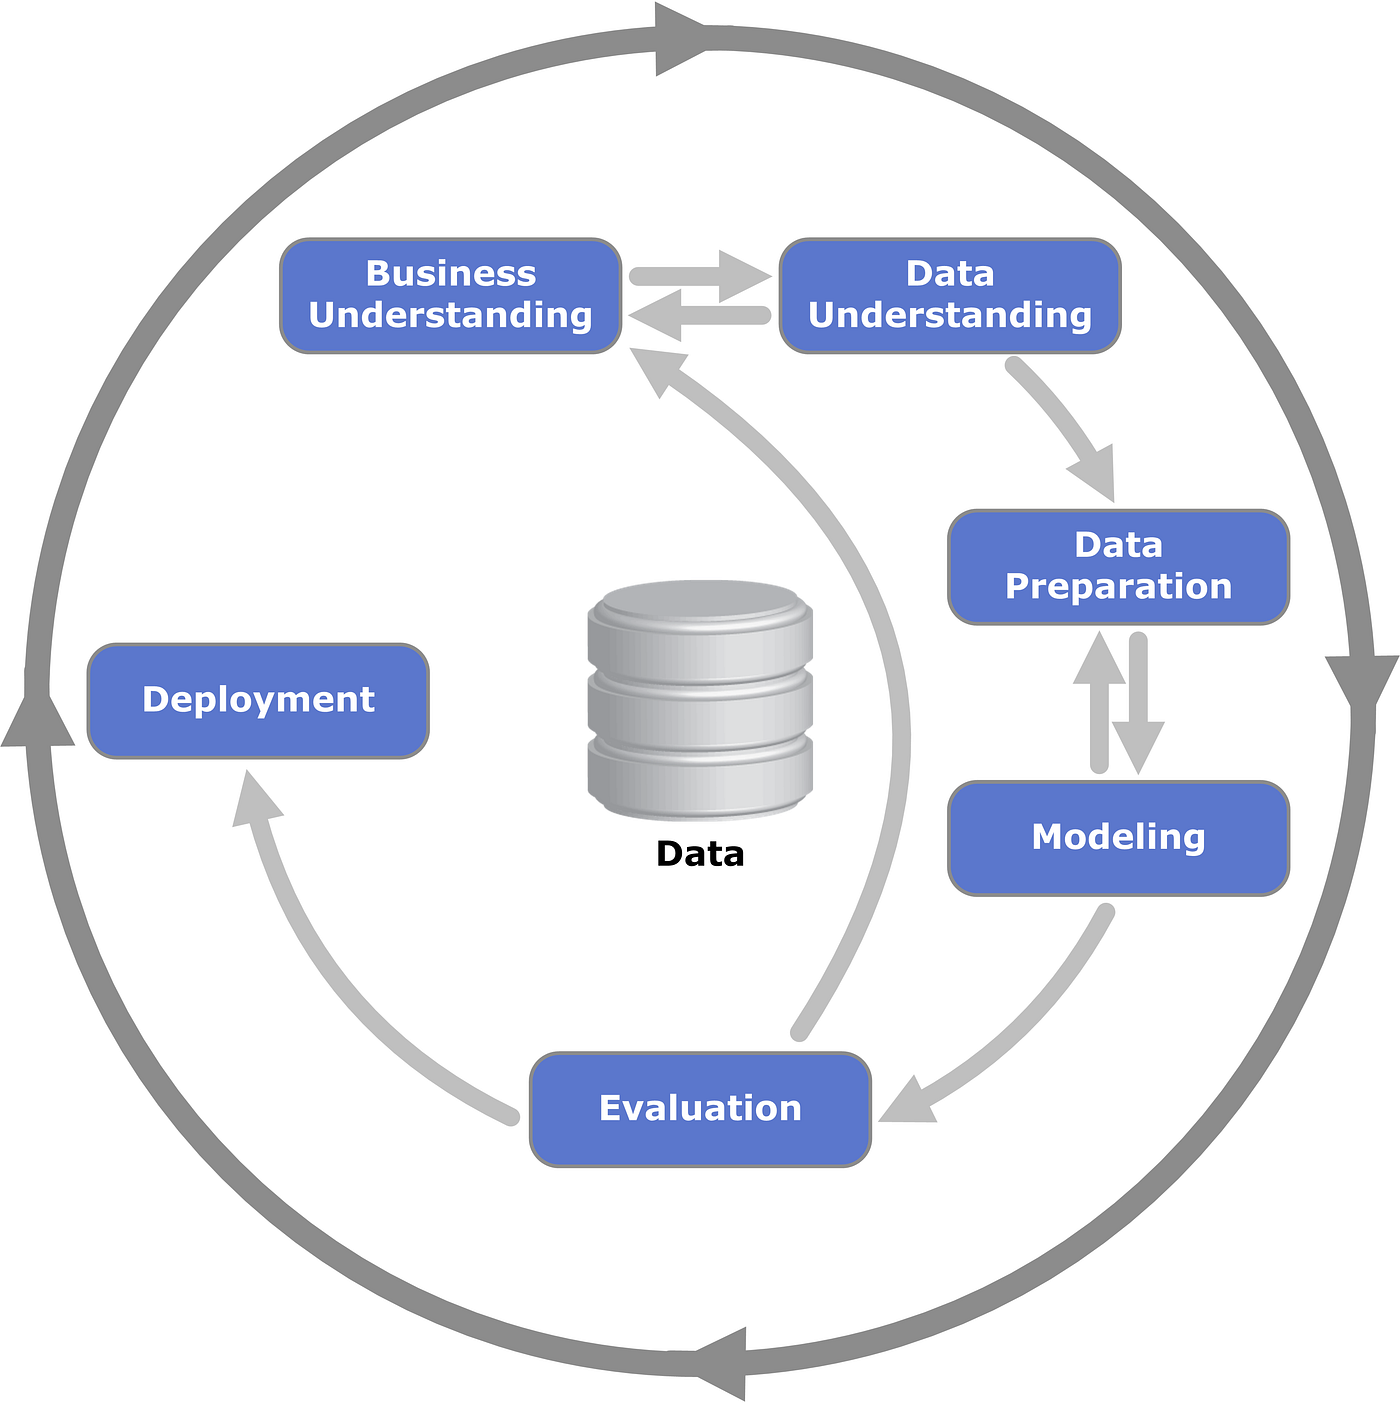
\includegraphics[width=0.9\textwidth]{../figures/CRISP-DM.png}
\end{figure}

\column{0.5\textwidth}
\begin{itemize}
    \item \textbf{Business Understanding:} Define objectives and requirements.
    \item \textbf{Data Understanding:} Explore and verify data quality.
    \item \textbf{Data Preparation:} Clean and preprocess data for modeling.
    \item \textbf{Modeling:} Build and evaluate predictive models.
    \item \textbf{Evaluation:} Assess model performance and alignment with goals.
    \item \textbf{Deployment:} Implement the model in a real-world environment.
\end{itemize}
\end{columns}
\end{frame}

%=============================================================================
\section{Business Understanding}
%=============================================================================

\begin{frame}{Business Problem}
\begin{block}{The Challenge}
Predict Peak Ground Acceleration (PGA) at any location in Italy given earthquake parameters for:
\begin{itemize}
    \item Seismic hazard assessment
    \item Emergency response planning
    \item Insurance risk modeling
\end{itemize}
\end{block}

\vspace{0.3cm}
\textbf{\textcolor{successgreen}{Goals}}
\begin{itemize}
    \item Early warning systems
    \item Physics-aware predictions
    \item Interpretable models
\end{itemize}
\end{frame}

%=============================================================================
\section{Data Understanding}
%=============================================================================

\begin{frame}{Dataset Overview: ITA18 Italian Strong-Motion Database}
\begin{columns}[T]
\column{0.5\textwidth}
\begin{table}
\centering
\small
\begin{tabular}{@{}ll@{}}
\toprule
\textbf{Attribute} & \textbf{Value} \\
\midrule
Total Records & 5,743 \\
Unique Events & 155 \\
Unique Stations & 1,650 \\
Temporal Coverage & 1976--2016 \\
Magnitude Range & $M_w$ 3.5--8.0 \\
Total Variables & 256 columns \\
\bottomrule
\end{tabular}
\end{table}

\vspace{0.2cm}
\textbf{Data Source:} INGV Engineering Strong Motion Database (ESM-db)

\column{0.5\textwidth}
\textbf{Variable Categories:}
\begin{itemize}
    \item \textbf{Source Parameters:} $M_w$, depth, strike, dip, rake, fault mechanism
    \item \textbf{Path/Distance Metrics:} epicentral, Joyner-Boore, rupture, Rx, Ry0
    \item \textbf{Site Characteristics:} $V_{s30}$, EC8 site class
    \item \textbf{Ground Motion Intensities:} PGA, PGV, spectral accelerations (SA)
\end{itemize}
\end{columns}

\vspace{0.3cm}
\begin{block}{Dataset Purpose}
Comprehensive Italian strong-motion database for ground motion prediction equation (GMPE) development and seismic hazard analysis.
\end{block}
\end{frame}

\begin{frame}{Train/Test Split: Temporal Horizon (Before EDA)}
\begin{columns}[T]
\column{0.45\textwidth}
\textbf{Training Set:}
\begin{itemize}
    \item 5,039 records (87.7\%), 150 events (96.8\%)
    \item May 6, 1976 $\rightarrow$ Oct 26, 2016
    \item Duration: 40.5 years
\end{itemize}

\vspace{0.5cm}
\textbf{Holdout Test Set:}
\begin{itemize}
    \item 704 records (12.3\%), 5 events (3.2\%)
    \item Oct 30, 2016 $\rightarrow$ Nov 13, 2016
    \item Duration: 14 days (most recent)
\end{itemize}

\begin{block}{Why Event-wise Train-Test Split?}
Prevent data leakage from same-event records appearing in train and test sets.
\end{block}

\column{0.45\textwidth}
\begin{alertblock}{Split Before EDA}
Prevents data leakage - all analysis on training data only.
\end{alertblock}

\vspace{0.4cm}
\textbf{Why Temporal Split?}
\begin{itemize}
    \item Simulates real deployment
    \item Train on 40-year history
    \item Test on future events
\end{itemize}

\vspace{0.4cm}
\textbf{ML Best Practice:}
\begin{itemize}
    \item No temporal information leakage
    \item Holdout for final evaluation only
    \item Events not split across sets
\end{itemize}
\end{columns}
\end{frame}

\begin{frame}{EDA: Magnitude and Depth Distributions (Training Data)}
\begin{figure}
\centering
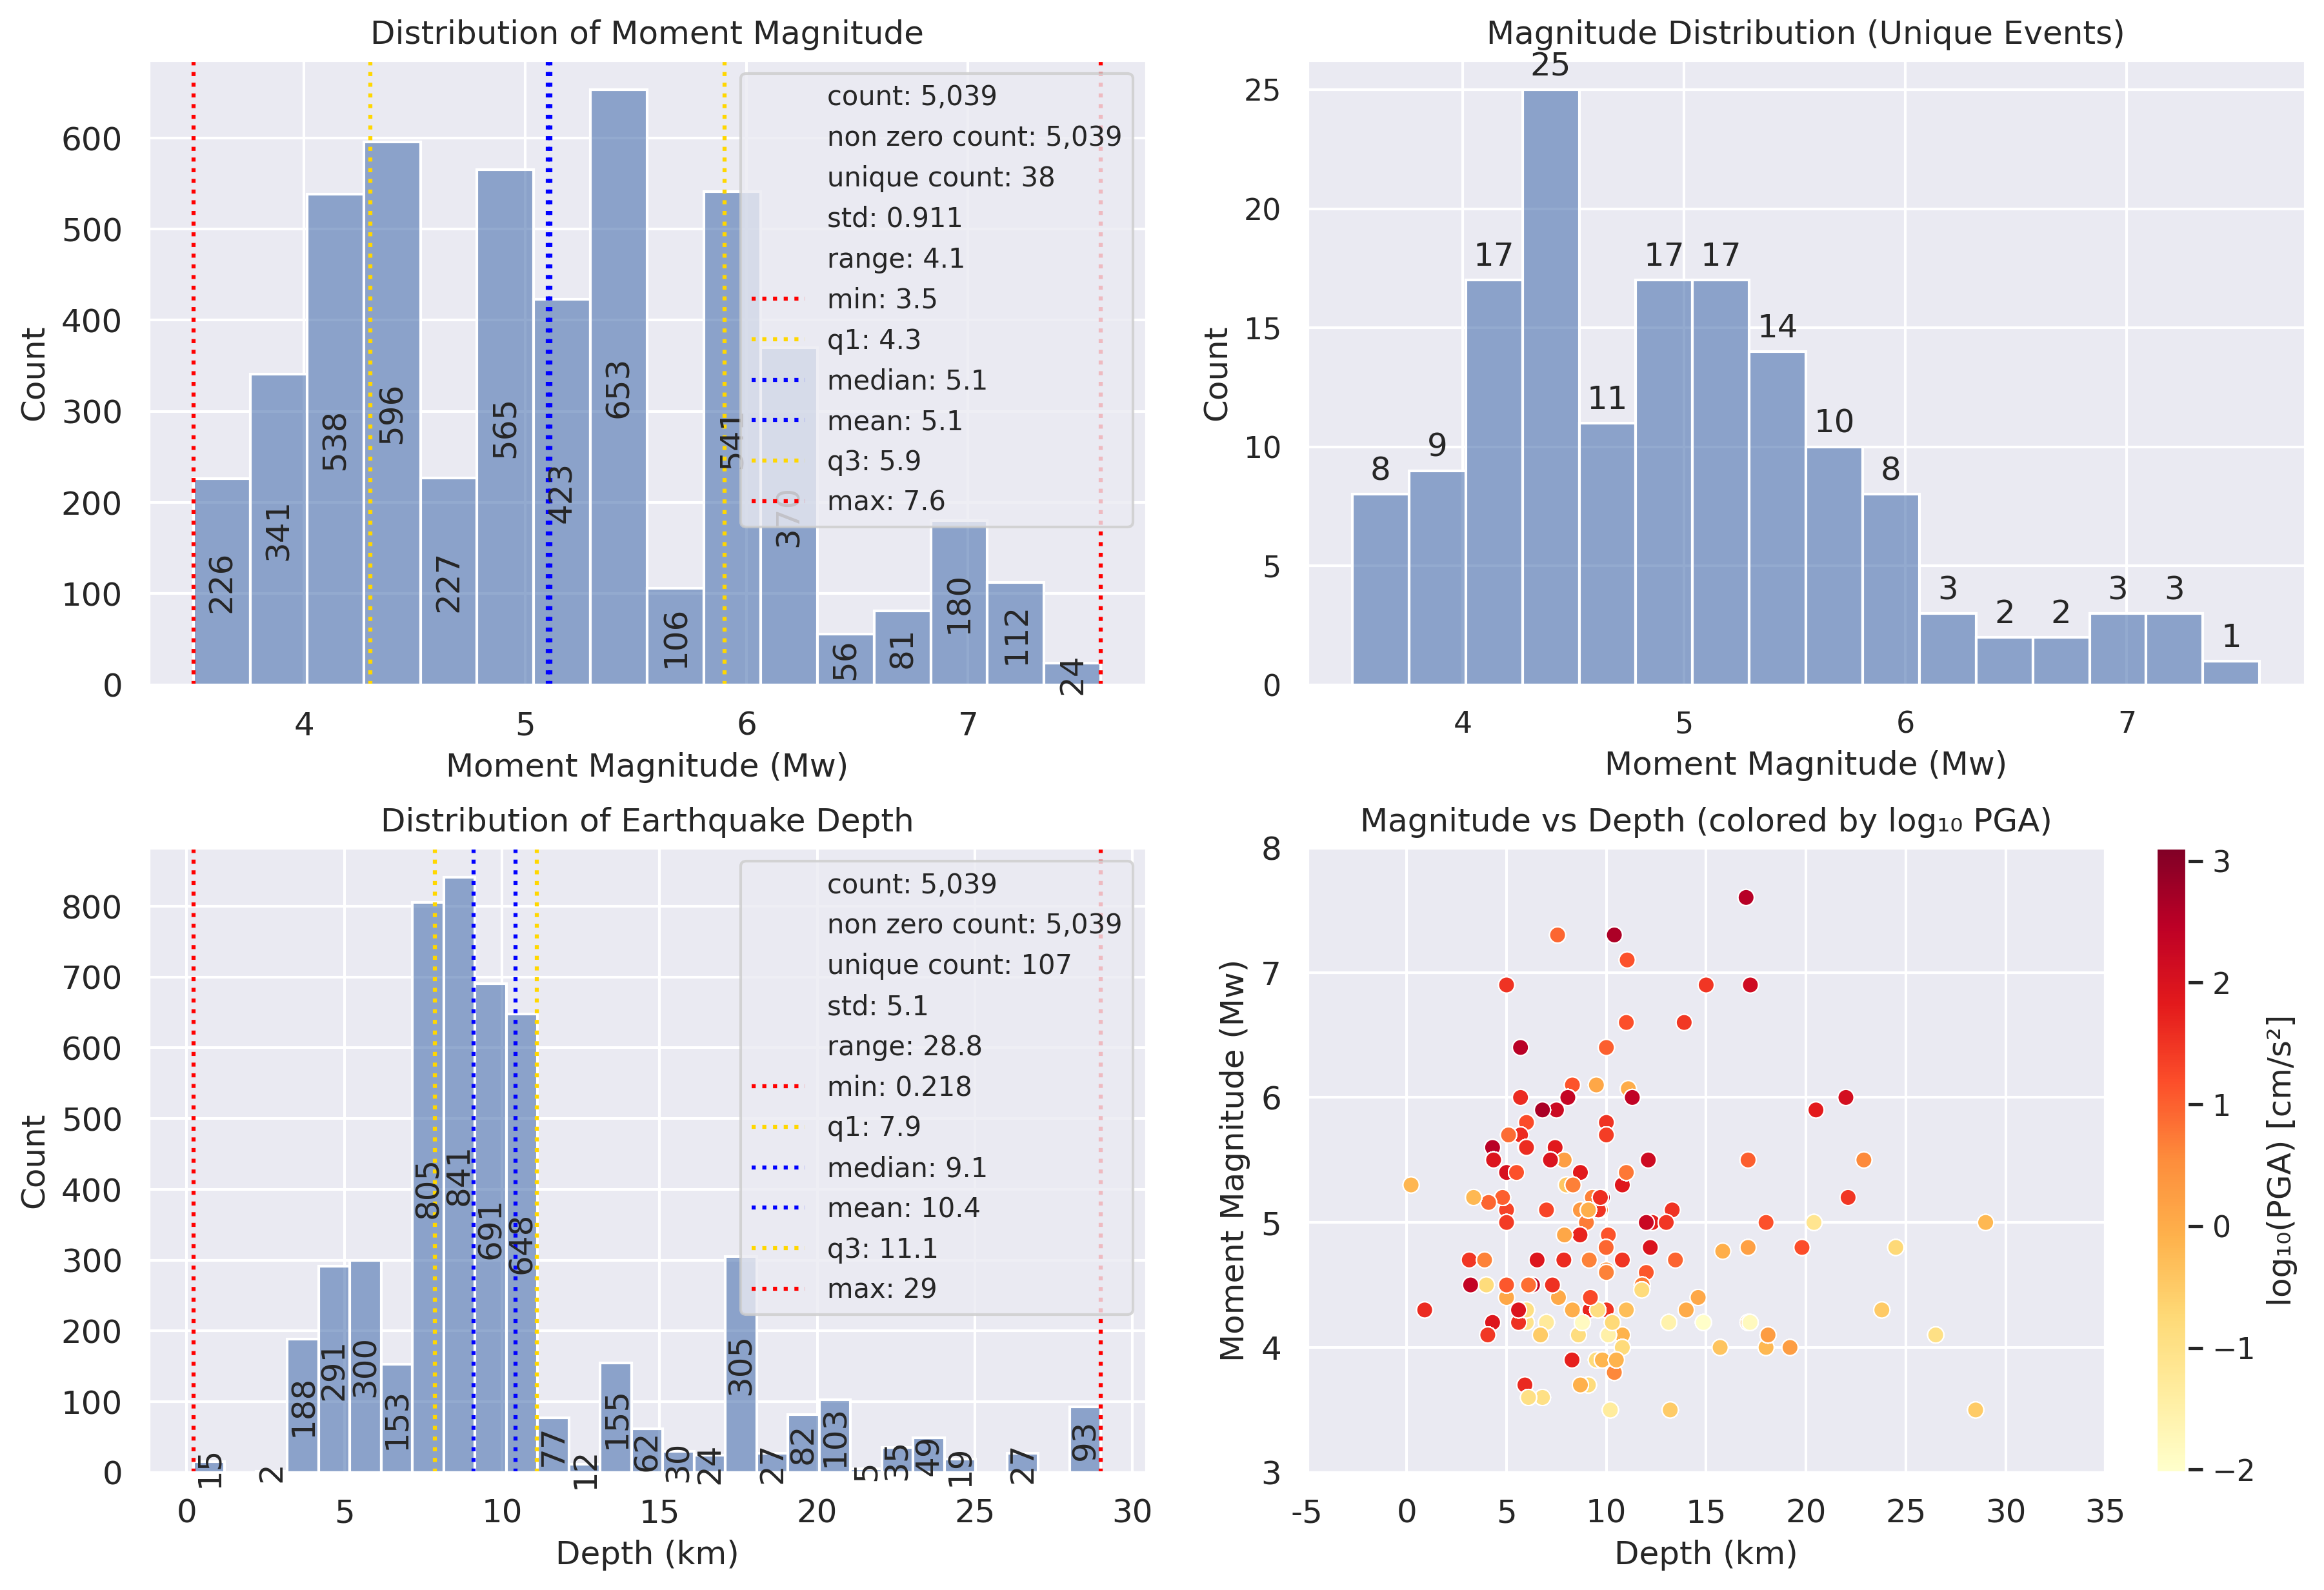
\includegraphics[width=0.7\textwidth]{../figures/eda/mw_depth_distributions.png}
\end{figure}
\end{frame}

\begin{frame}{EDA: Fault Mechanism Distribution (Training Data)}
\begin{figure}
\centering
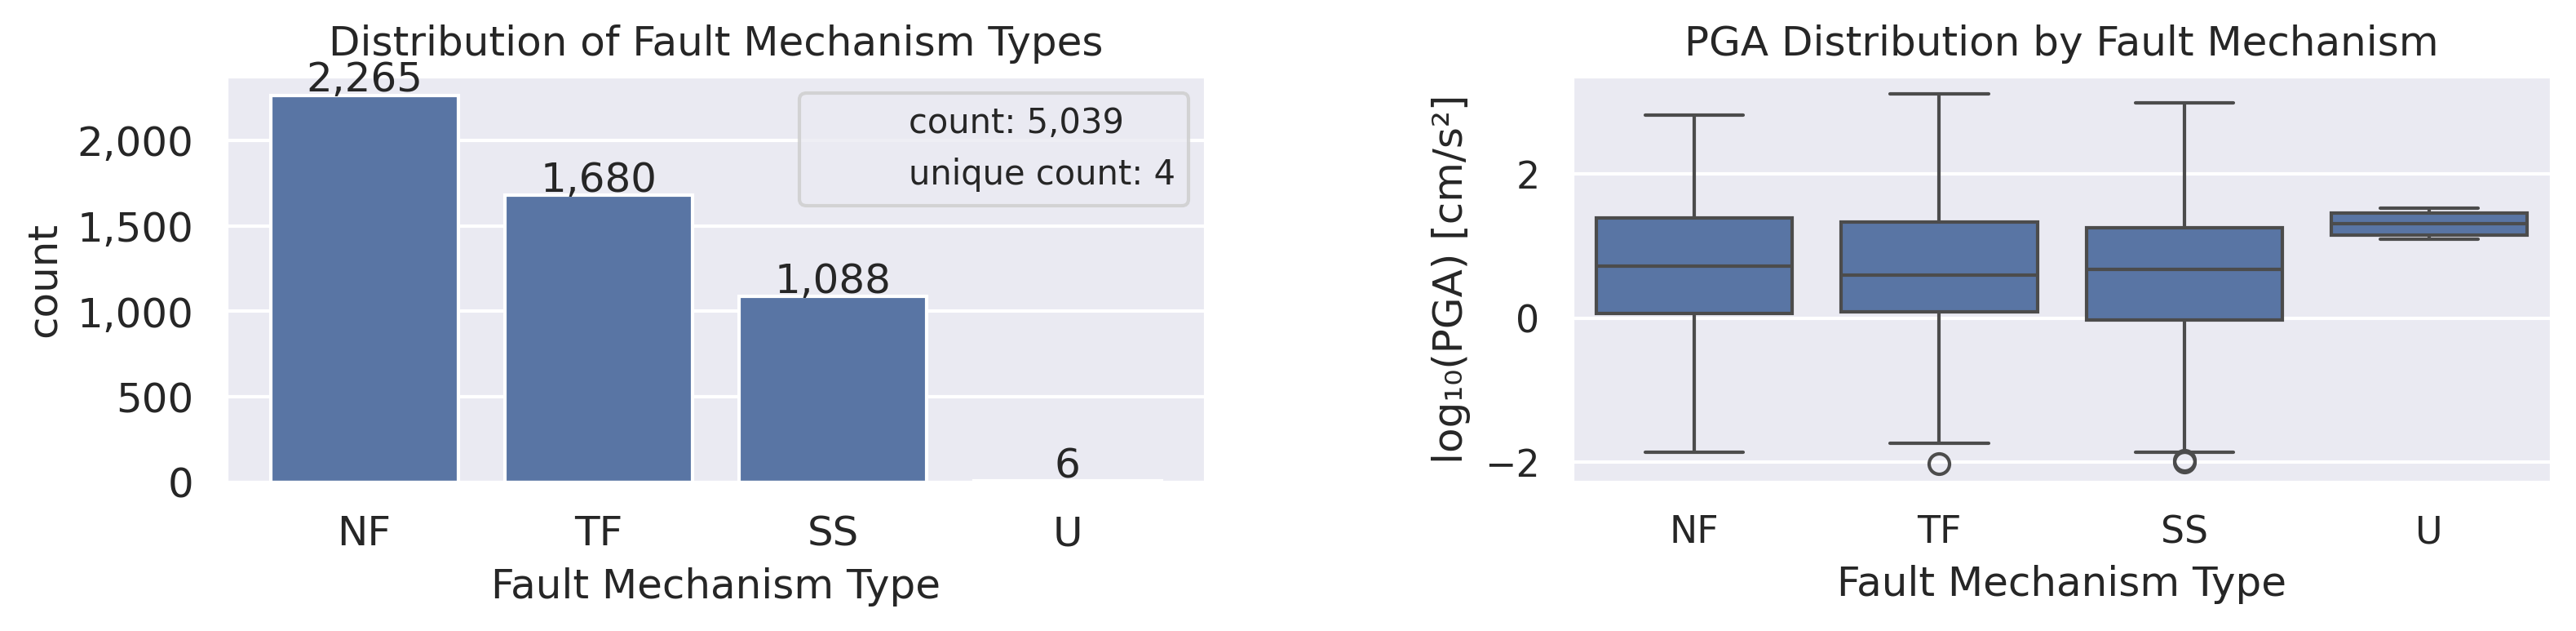
\includegraphics[width=1.0\textwidth]{../figures/eda/fault_mechanism_analysis.png}
\end{figure}

\textbf{Distribution:}
\begin{itemize}
    \item \textbf{NF:} 44.9\%, \textbf{TF:} 33.3\%, \textbf{SS:} 21.6\%, Unknown: 0.1\%
\end{itemize}
\end{frame}

\begin{frame}{EDA: Distance Metrics Analysis (Training Data)}
\begin{figure}
\centering
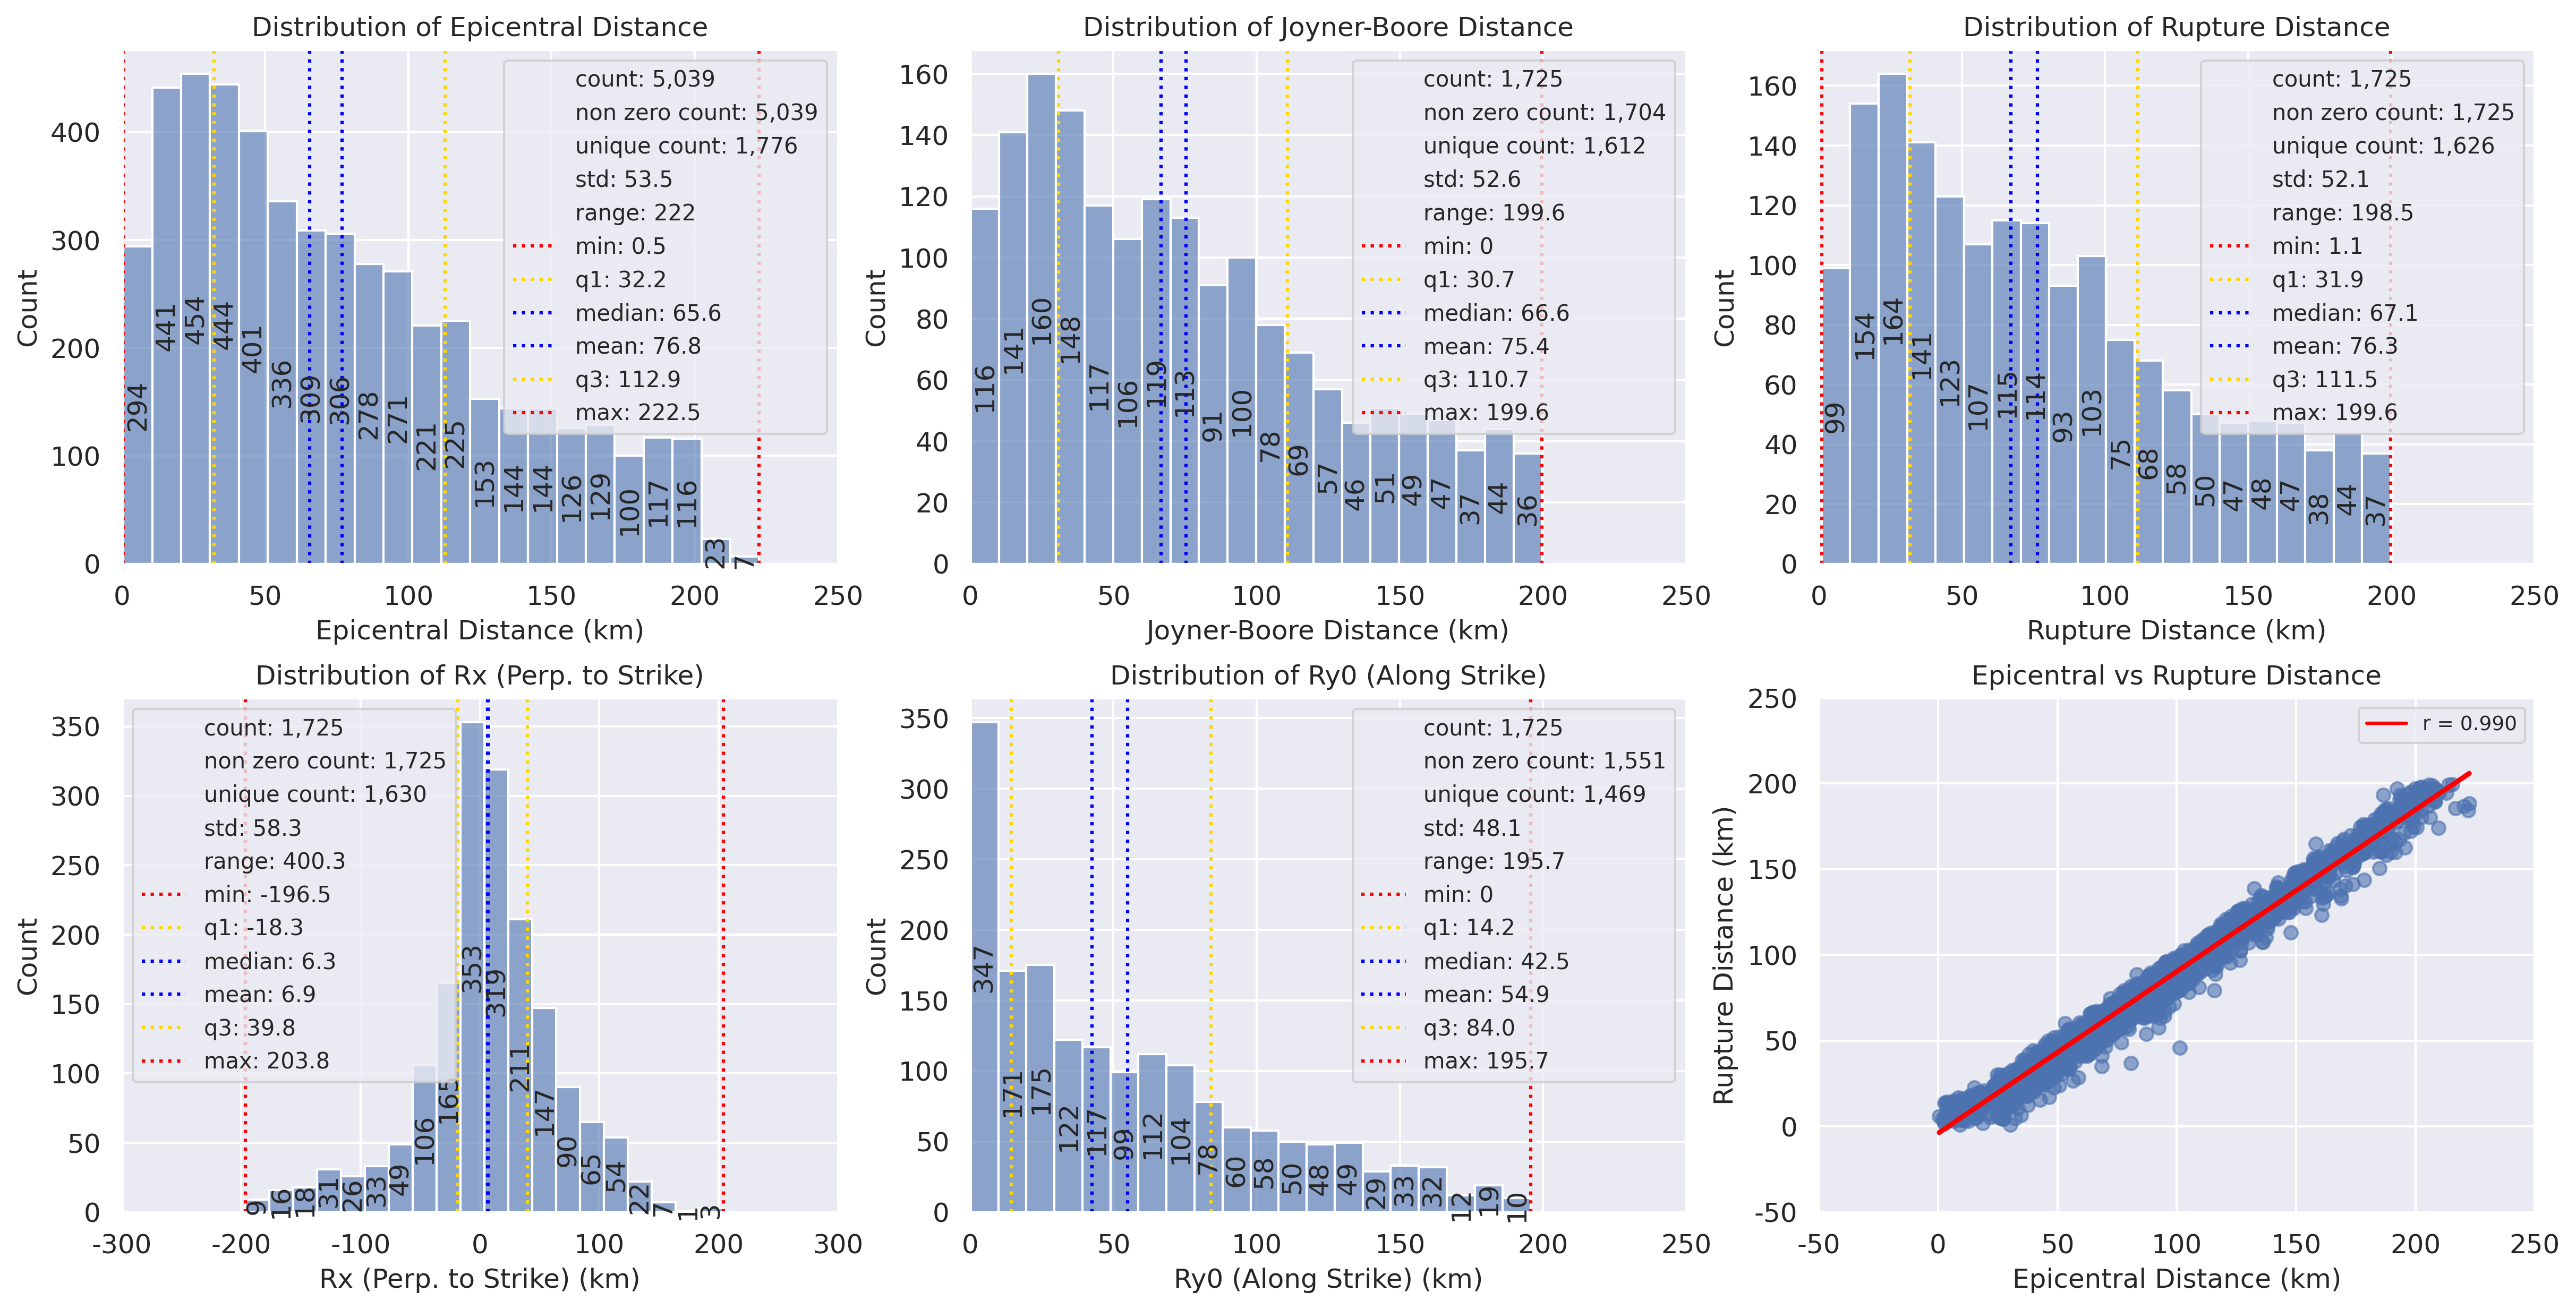
\includegraphics[width=1.0\textwidth]{../figures/eda/distance_distributions.png}
\end{figure}
\end{frame}

\begin{frame}{EDA: Ground Motion Attenuation Patterns (Training Data)}
\begin{figure}
\centering
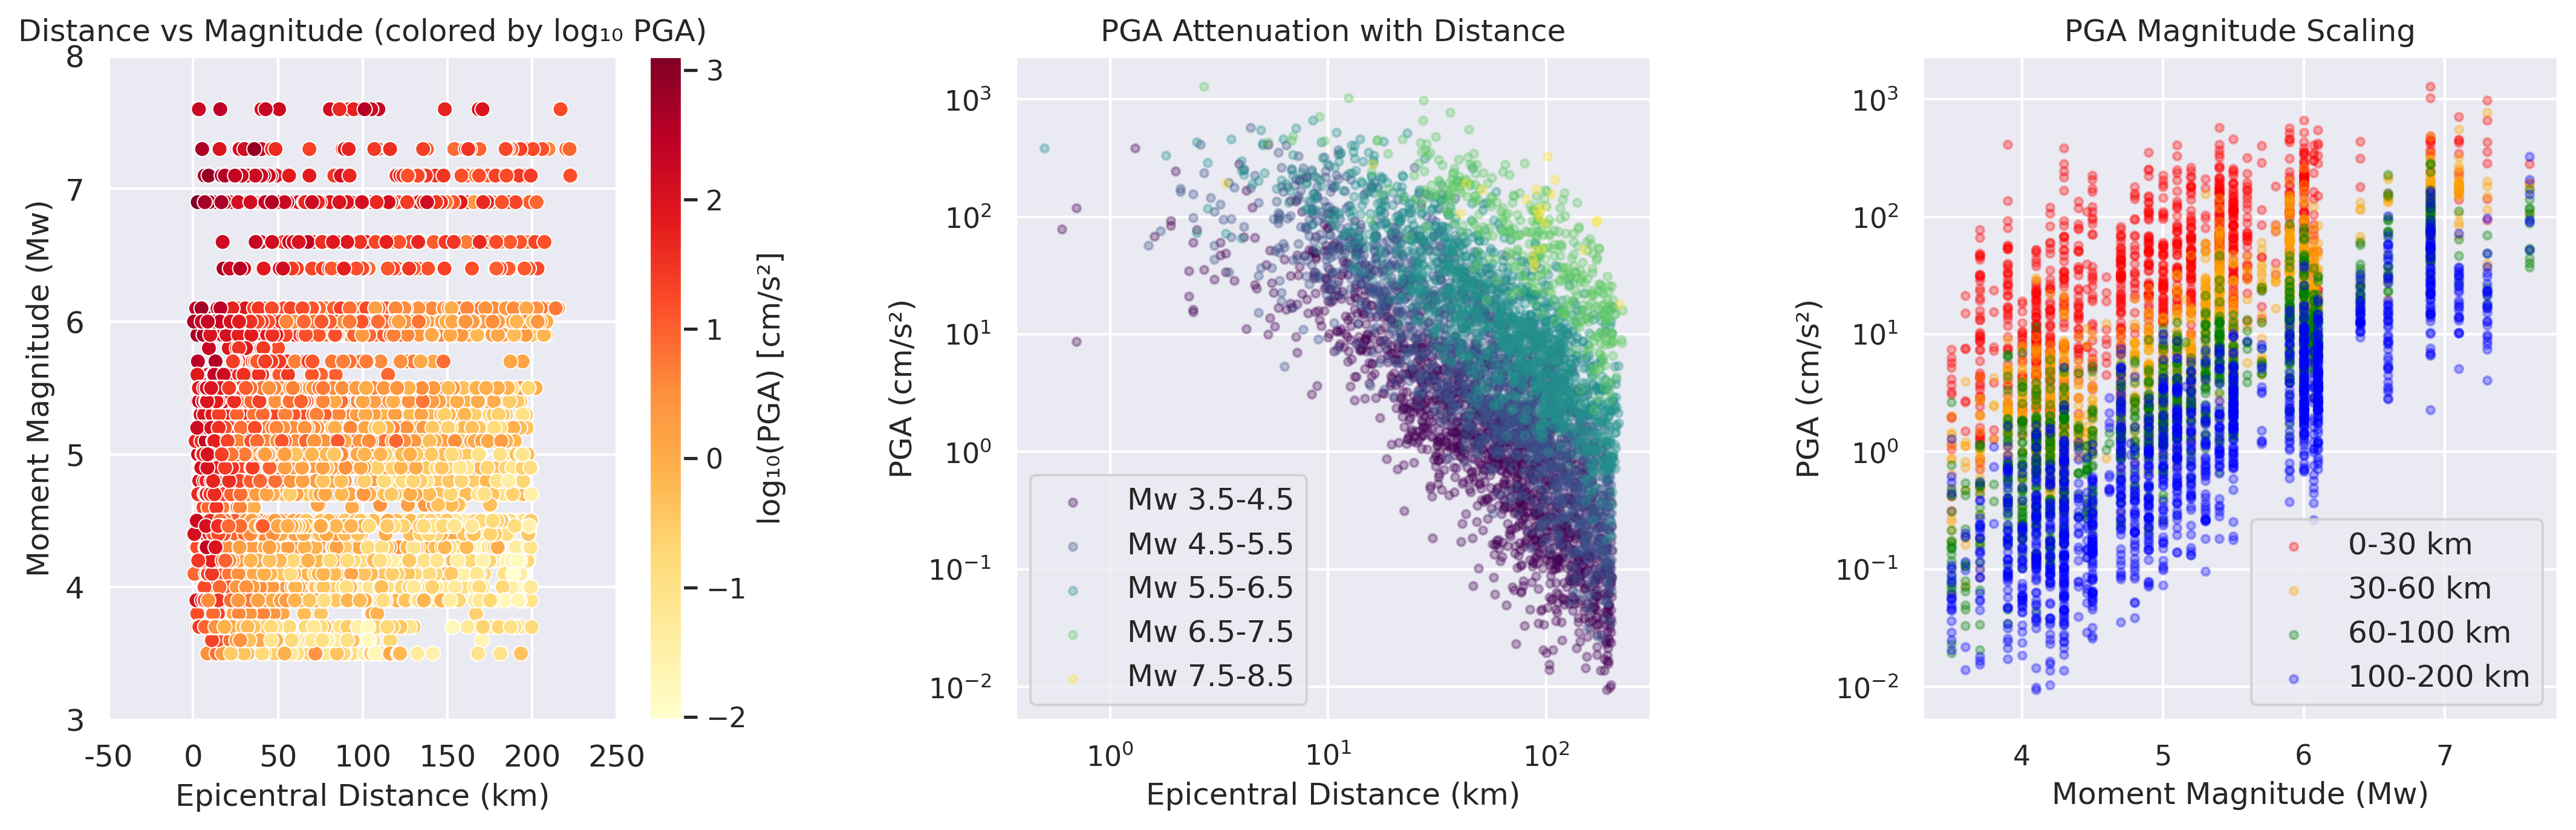
\includegraphics[width=0.85\textwidth]{../figures/eda/pga_attenuation_scaling.png}
\end{figure}

\textbf{Physical Observations:}
\begin{columns}[T]
\column{0.33\textwidth}
\begin{itemize}
    \item \textbf{Scatter:} Site effects, path variability
\end{itemize}

\column{0.33\textwidth}
\begin{itemize}
    \item \textbf{Distance Attenuation:}
    \item PGA $\downarrow$ with distance
\end{itemize}

\column{0.33\textwidth}
\begin{itemize}
    \item \textbf{Magnitude Scaling:}
    \item PGA $\uparrow$ with $M_w$
\end{itemize}
\end{columns}
\end{frame}

\begin{frame}{EDA: Site Conditions Analysis (Training Data)}
\begin{figure}
\centering
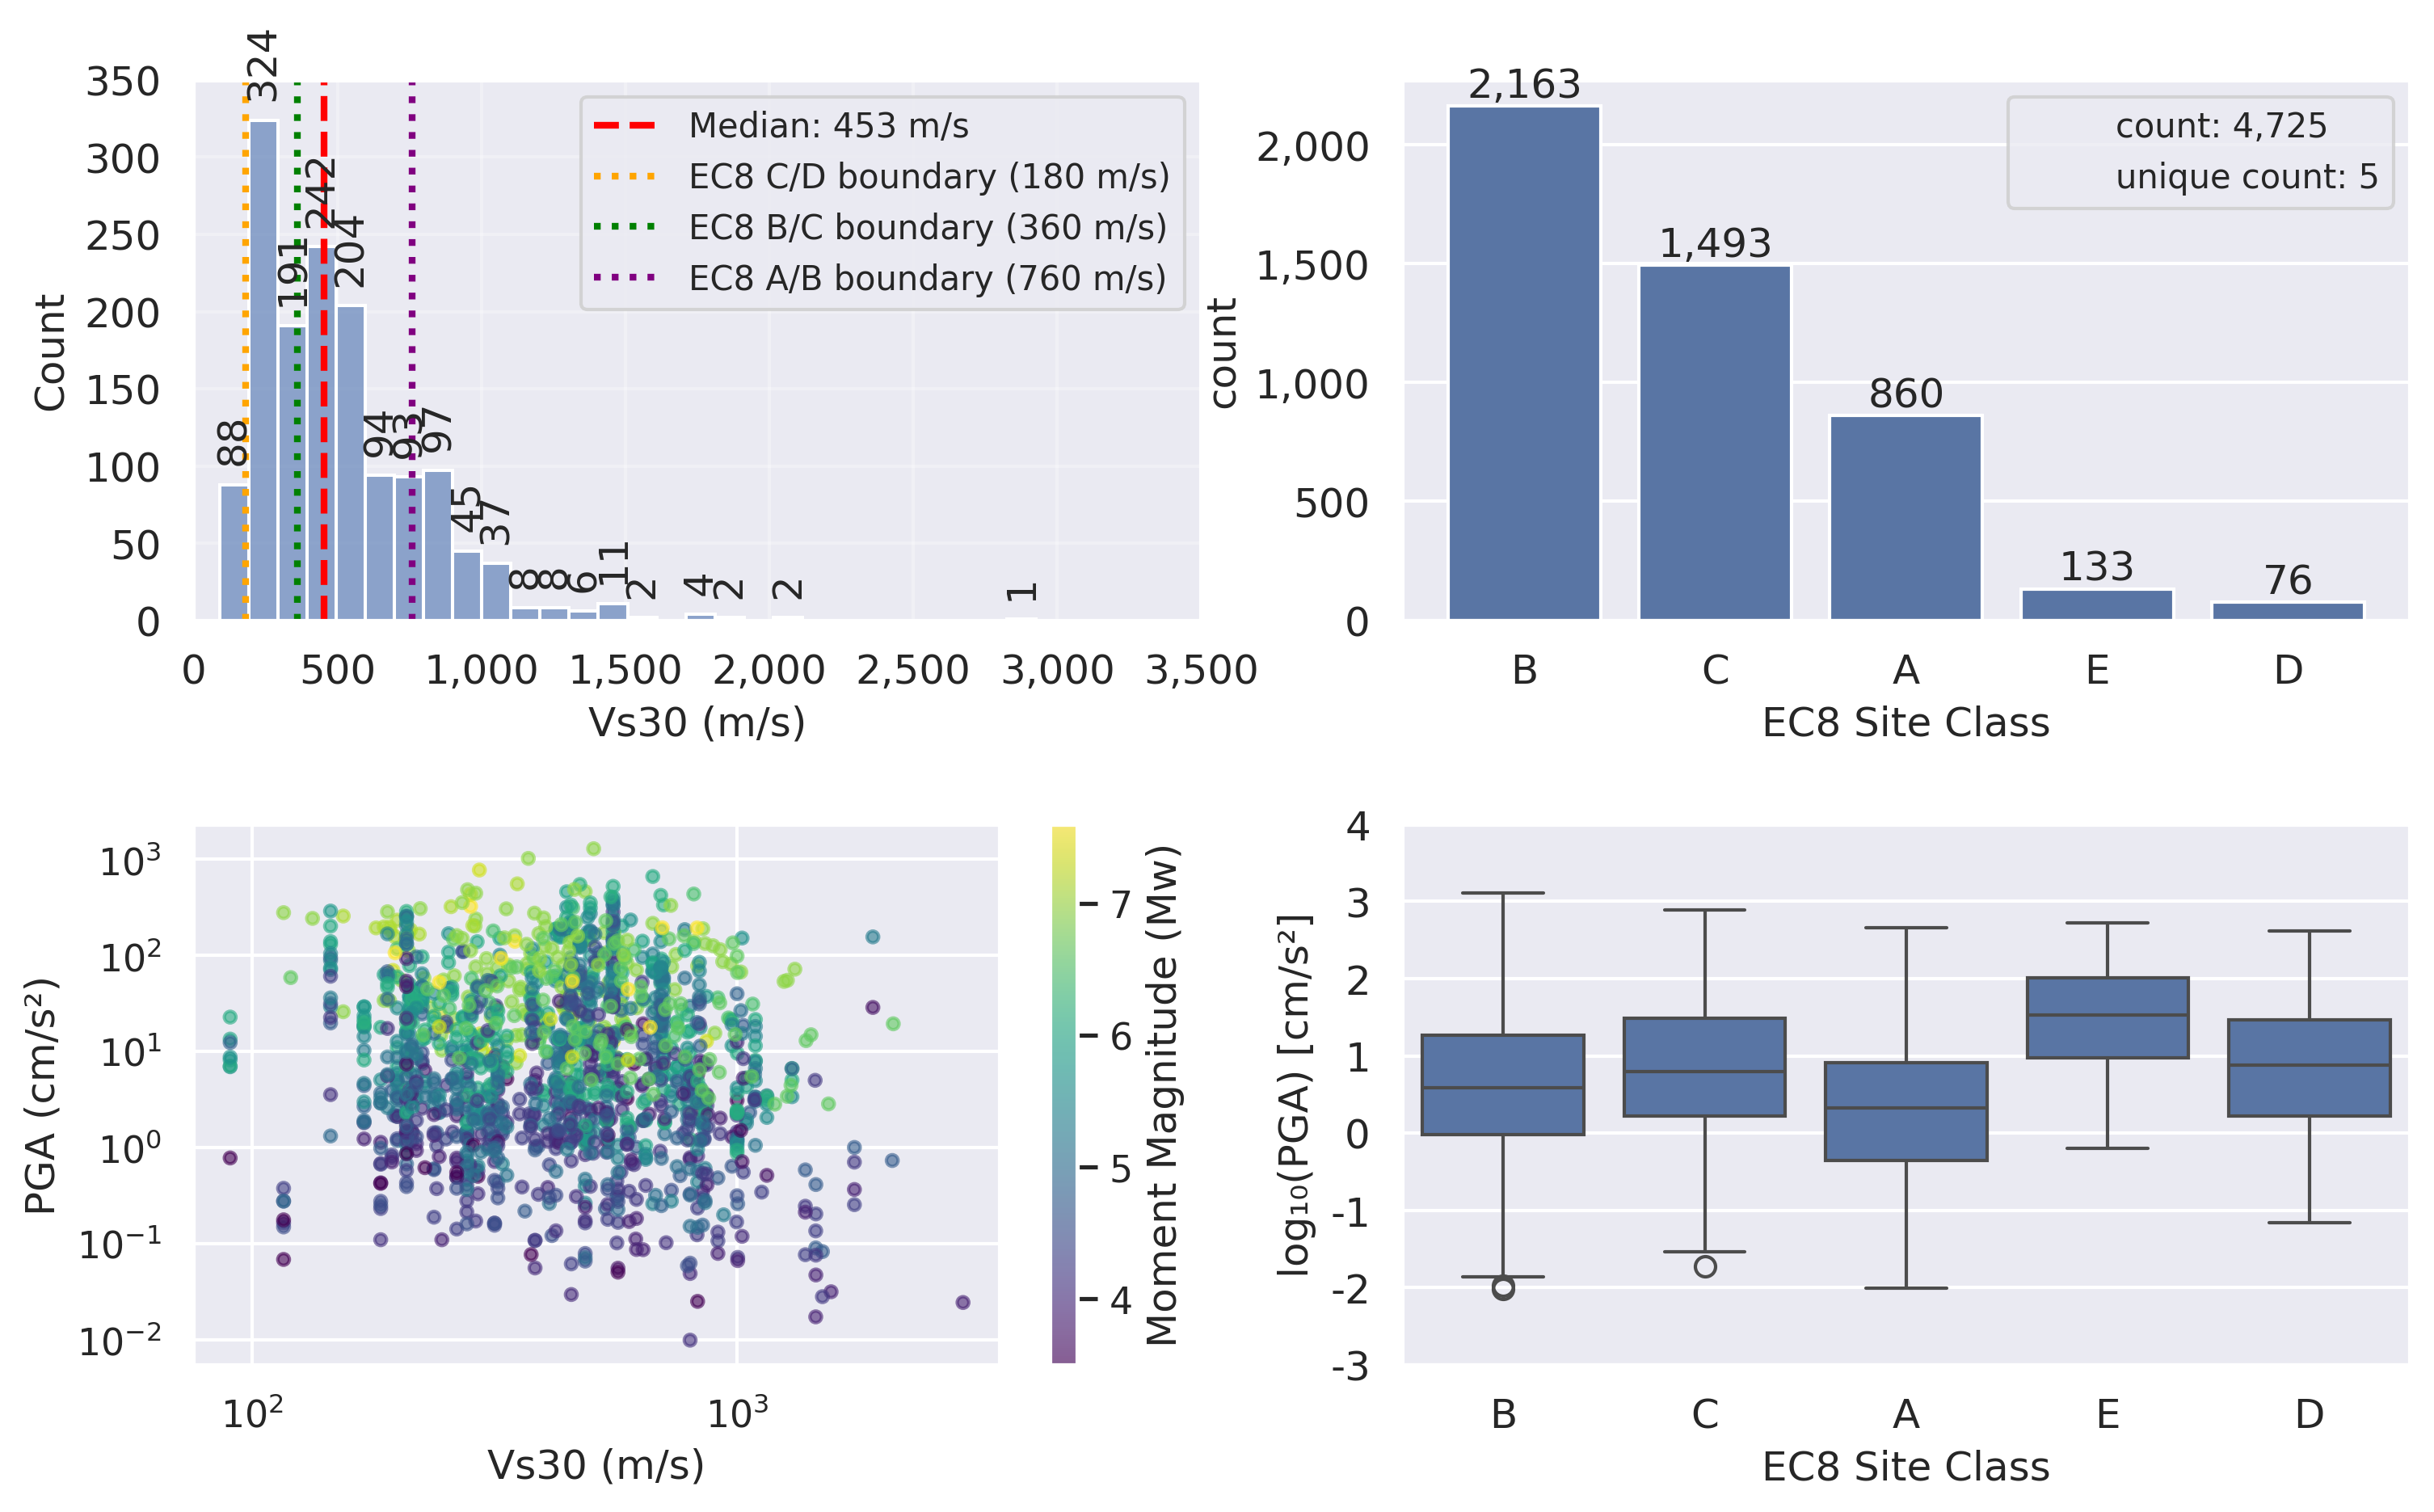
\includegraphics[width=0.65\textwidth]{../figures/eda/site_conditions_analysis.png}
\end{figure}

\begin{columns}[T]
\column{0.5\textwidth}
\textbf{Key:} Lower $V_{s30}$ $\rightarrow$ higher PGA (soil amplification)

\column{0.5\textwidth}
\textbf{EC8 Classes:} A: 4.3\%, B: 11.3\%, C: 9.4\%, D: 1.1\%, E: 2.6\%
\end{columns}
\end{frame}

\begin{frame}{EDA: Ground Motion Distributions (Training Data)}
\begin{figure}
\centering
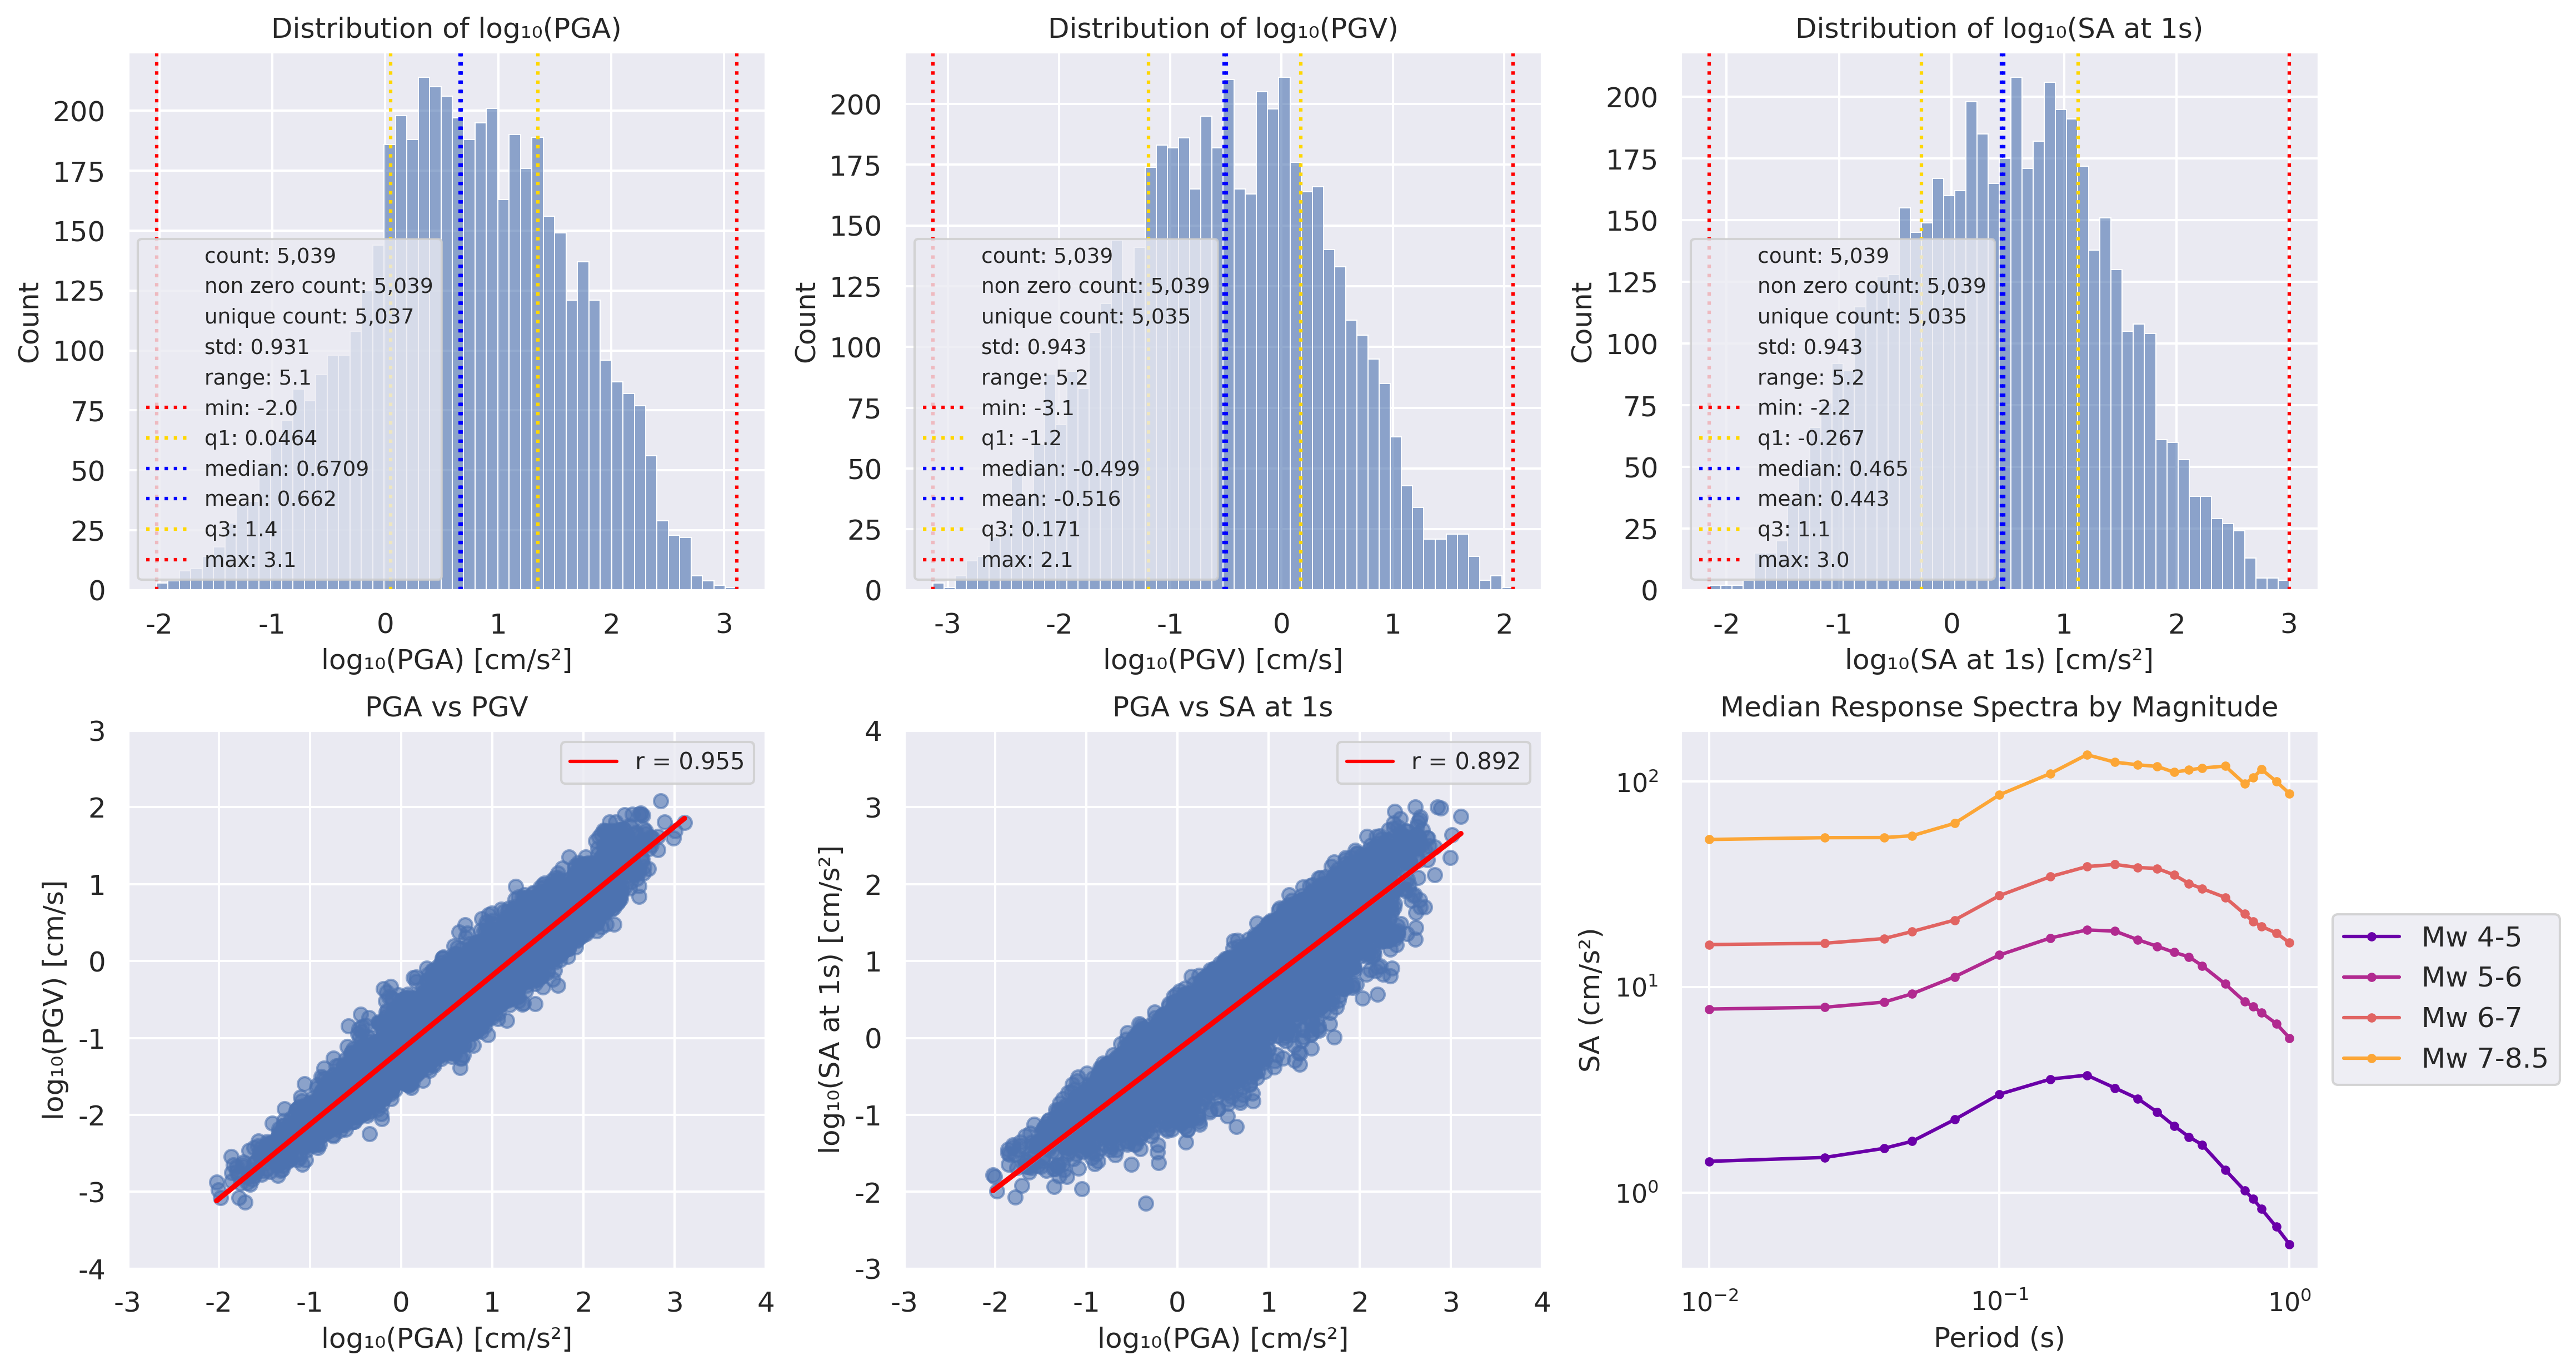
\includegraphics[width=0.9\textwidth]{../figures/eda/ground_motion_distributions.png}
\end{figure}
\end{frame}

\begin{frame}{Initial Features for Modeling}
\begin{columns}[T]
\column{0.33\textwidth}
\textbf{Source Parameters (6)}
\begin{itemize}
    \item $M_w$ (moment magnitude)
    \item ev\_depth\_km (hypocentral)
    \item fm\_type\_code (fault mechanism)
    \item es\_strike (strike angle)
    \item es\_dip (dip angle)
    \item es\_rake (rake angle)
\end{itemize}

\column{0.33\textwidth}
\textbf{Distance Metrics (5)}
\begin{itemize}
    \item epi\_dist (epicentral)
    \item JB\_dist (Joyner-Boore)
    \item rup\_dist (rupture)
    \item Rx\_dist (horizontal)
    \item Ry0\_dist (parallel)
\end{itemize}

\column{0.33\textwidth}
\textbf{Site Parameters (2)}
\begin{itemize}
    \item vs30\_m\_sec (shear wave vel.)
    \item ec8\_code (site class)
\end{itemize}
\end{columns}

\vspace{0.3cm}
\begin{block}{Target Variable}
rotD50\_pga (Peak Ground Acceleration) $\rightarrow$ $\log_{10}$(PGA) for modeling
\end{block}
\vspace{0.2cm}
\centering
\textbf{Total: 13 candidate features $\rightarrow$ Need systematic filtering}
\end{frame}

%=============================================================================
\section{Data Preparation}
%=============================================================================

\begin{frame}{Categorical Encoding Strategy}
\textbf{Ordinal Encoding}

\vspace{0.3cm}
\begin{columns}[T]
\column{0.48\textwidth}
\textbf{Fault Mechanism} (fm\_type\_code)
\begin{table}
\centering
\small
\begin{tabular}{@{}lc@{}}
\toprule
\textbf{Type} & \textbf{Encoded} \\
\midrule
Normal (NF) & 0 \\
Unknown (U) & 0 \\
Strike-Slip (SS) & 1 \\
Thrust (TF) & 2 \\
\bottomrule
\end{tabular}
\end{table}

\column{0.48\textwidth}
\textbf{EC8 Site Class} (ec8\_code)
\begin{table}
\centering
\small
\begin{tabular}{@{}lc@{}}
\toprule
\textbf{Class} & \textbf{Encoded} \\
\midrule
A (Rock) & 0 \\
B & 1 \\
C & 2 \\
D & 3 \\
E (Soft soil) & 4 \\
\bottomrule
\end{tabular}
\end{table}
\end{columns}

\vspace{0.3cm}
\textbf{Encoding Strategy:}
\begin{itemize}
    \item FM: NF and U grouped as baseline (0)
    \item EC8: Natural ordering from hard to soft soil
    \item New features: \texttt{fm\_encoded}, \texttt{ec8\_encoded}
\end{itemize}
\end{frame}

\begin{frame}{Step 1: Missing Data Analysis}
\begin{columns}[T]
\column{0.5\textwidth}
\textbf{Availability by Variable:}
\begin{table}
\centering
\scriptsize
\begin{tabular}{@{}lrr@{}}
\toprule
\textbf{Variable} & \textbf{Missing \%} & \textbf{Action} \\
\midrule
$M_w$, epi\_dist, depth & 0\% & Keep \\
fm\_encoded & 0\% & Keep \\
$V_{s30}$ & 71\% & Impute \\
es\_strike, dip, rake & 66-67\% & Drop \\
JB, rup, Rx, Ry0 & 66\% & Drop \\
ec8\_code & 6\% & Drop \\
\bottomrule
\end{tabular}
\end{table}

\vspace{0.3cm}
\textbf{Imputation Strategy:}
\begin{itemize}
    \item $V_{s30}$: median = 453 m/s (EC8 class B/C boundary)
\end{itemize}

\column{0.5\textwidth}
\textbf{Exclusion Rationale:}
\begin{itemize}
    \item \textbf{es\_strike/dip/rake:} 66-67\% missing, complex effects, \texttt{fm\_encoded} captures mechanism
    \item \textbf{JB/rup/Rx/Ry0:} 66\% missing, only for finite-fault events
    \item \textbf{ec8\_code:} Redundant with $V_{s30}$ (both represent site conditions)
\end{itemize}

\vspace{0.2cm}
\textcolor{alertred}{\textbf{Filtered: 8 variables removed}}
\end{columns}
\end{frame}

\begin{frame}{Step 2: Feature Engineering (Log Transforms)}
\begin{columns}[T]
\column{0.48\textwidth}
\textbf{Epicentral Distance:}
\begin{equation*}
\log_{10}(R_{epi} + 1)
\end{equation*}
\textbf{Why?}
\begin{itemize}
    \item Linearizes geometric spreading ($\propto 1/R$)
    \item $+1$ prevents undefined at $R=0$
    \item Better relationship with log(PGA)
\end{itemize}

\column{0.48\textwidth}
\textbf{Site Condition ($V_{s30}$):}
\begin{equation*}
\log_{10}(V_{s30})
\end{equation*}
\textbf{Why?}
\begin{itemize}
    \item Captures multiplicative site amplification
    \item Maps soil stiffness to response
    \item Linear relationship with log(PGA)
\end{itemize}
\end{columns}

\vspace{0.3cm}
\textbf{Result:} Created \texttt{log\_epi\_dist} and \texttt{log\_vs30} features
\end{frame}

\begin{frame}{Step 3: Correlation Analysis}
\begin{figure}
\centering
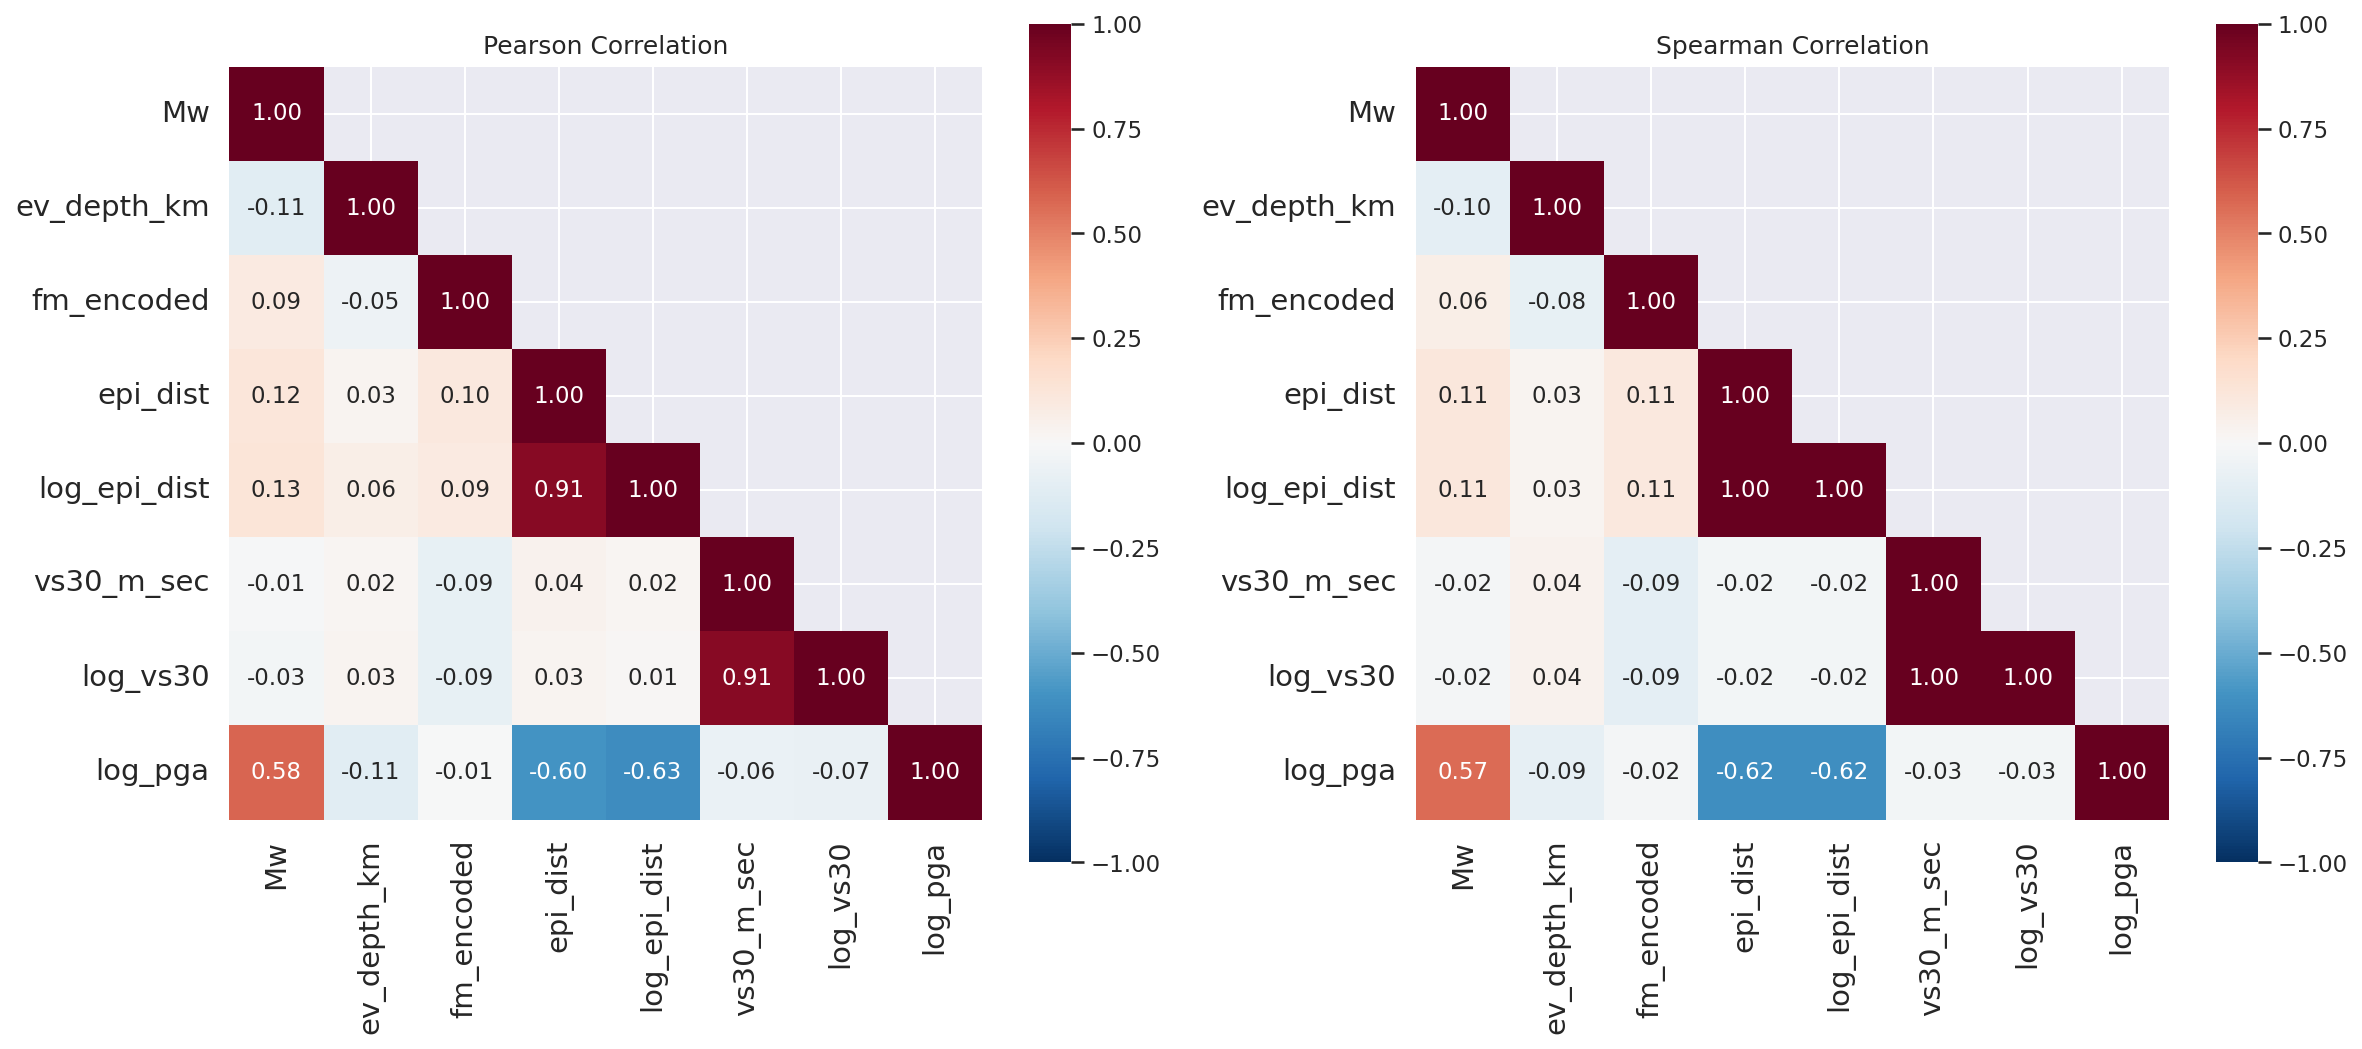
\includegraphics[width=0.95\textwidth]{../figures/eda/correlation_matrix.png}
\caption{Pearson (left) \& Spearman (right) Correlation Matrices}
\end{figure}
\end{frame}

\begin{frame}{Step 3: Correlation Analysis -- Findings}
\textbf{High Correlations Detected ($|r| > 0.7$):}
\vspace{0.2cm}

\begin{columns}[T]
\column{0.48\textwidth}
\begin{table}
\centering
\begin{tabular}{@{}lc@{}}
\toprule
\textbf{Feature Pair} & \textbf{Pearson $r$} \\
\midrule
epi\_dist $\leftrightarrow$ log\_epi\_dist & 0.908 \\
vs30\_m\_sec $\leftrightarrow$ log\_vs30 & 0.912 \\
\bottomrule
\end{tabular}
\end{table}

\vspace{0.3cm}
\begin{alertblock}{Why This Matters}
High correlation causes multicollinearity $\rightarrow$ redundant information
\end{alertblock}

\column{0.48\textwidth}
\textbf{Decision Rules:}
\begin{enumerate}
    \item \textcolor{alertred}{Drop} original features
    \item \textcolor{successgreen}{Keep} log-transformed versions
    \item Reason: Better linearity with log(PGA)
\end{enumerate}

\vspace{0.3cm}
\textbf{Features Removed:}
\begin{itemize}
    \item[$\times$] epi\_dist
    \item[$\times$] vs30\_m\_sec
\end{itemize}

\textbf{Features Retained:}
\begin{itemize}
    \item[\checkmark] log\_epi\_dist
    \item[\checkmark] log\_vs30
\end{itemize}
\end{columns}
\end{frame}

\begin{frame}{Step 4: VIF Analysis (Multicollinearity Check)}
\begin{columns}[T]
\column{0.5\textwidth}
\begin{figure}
\centering
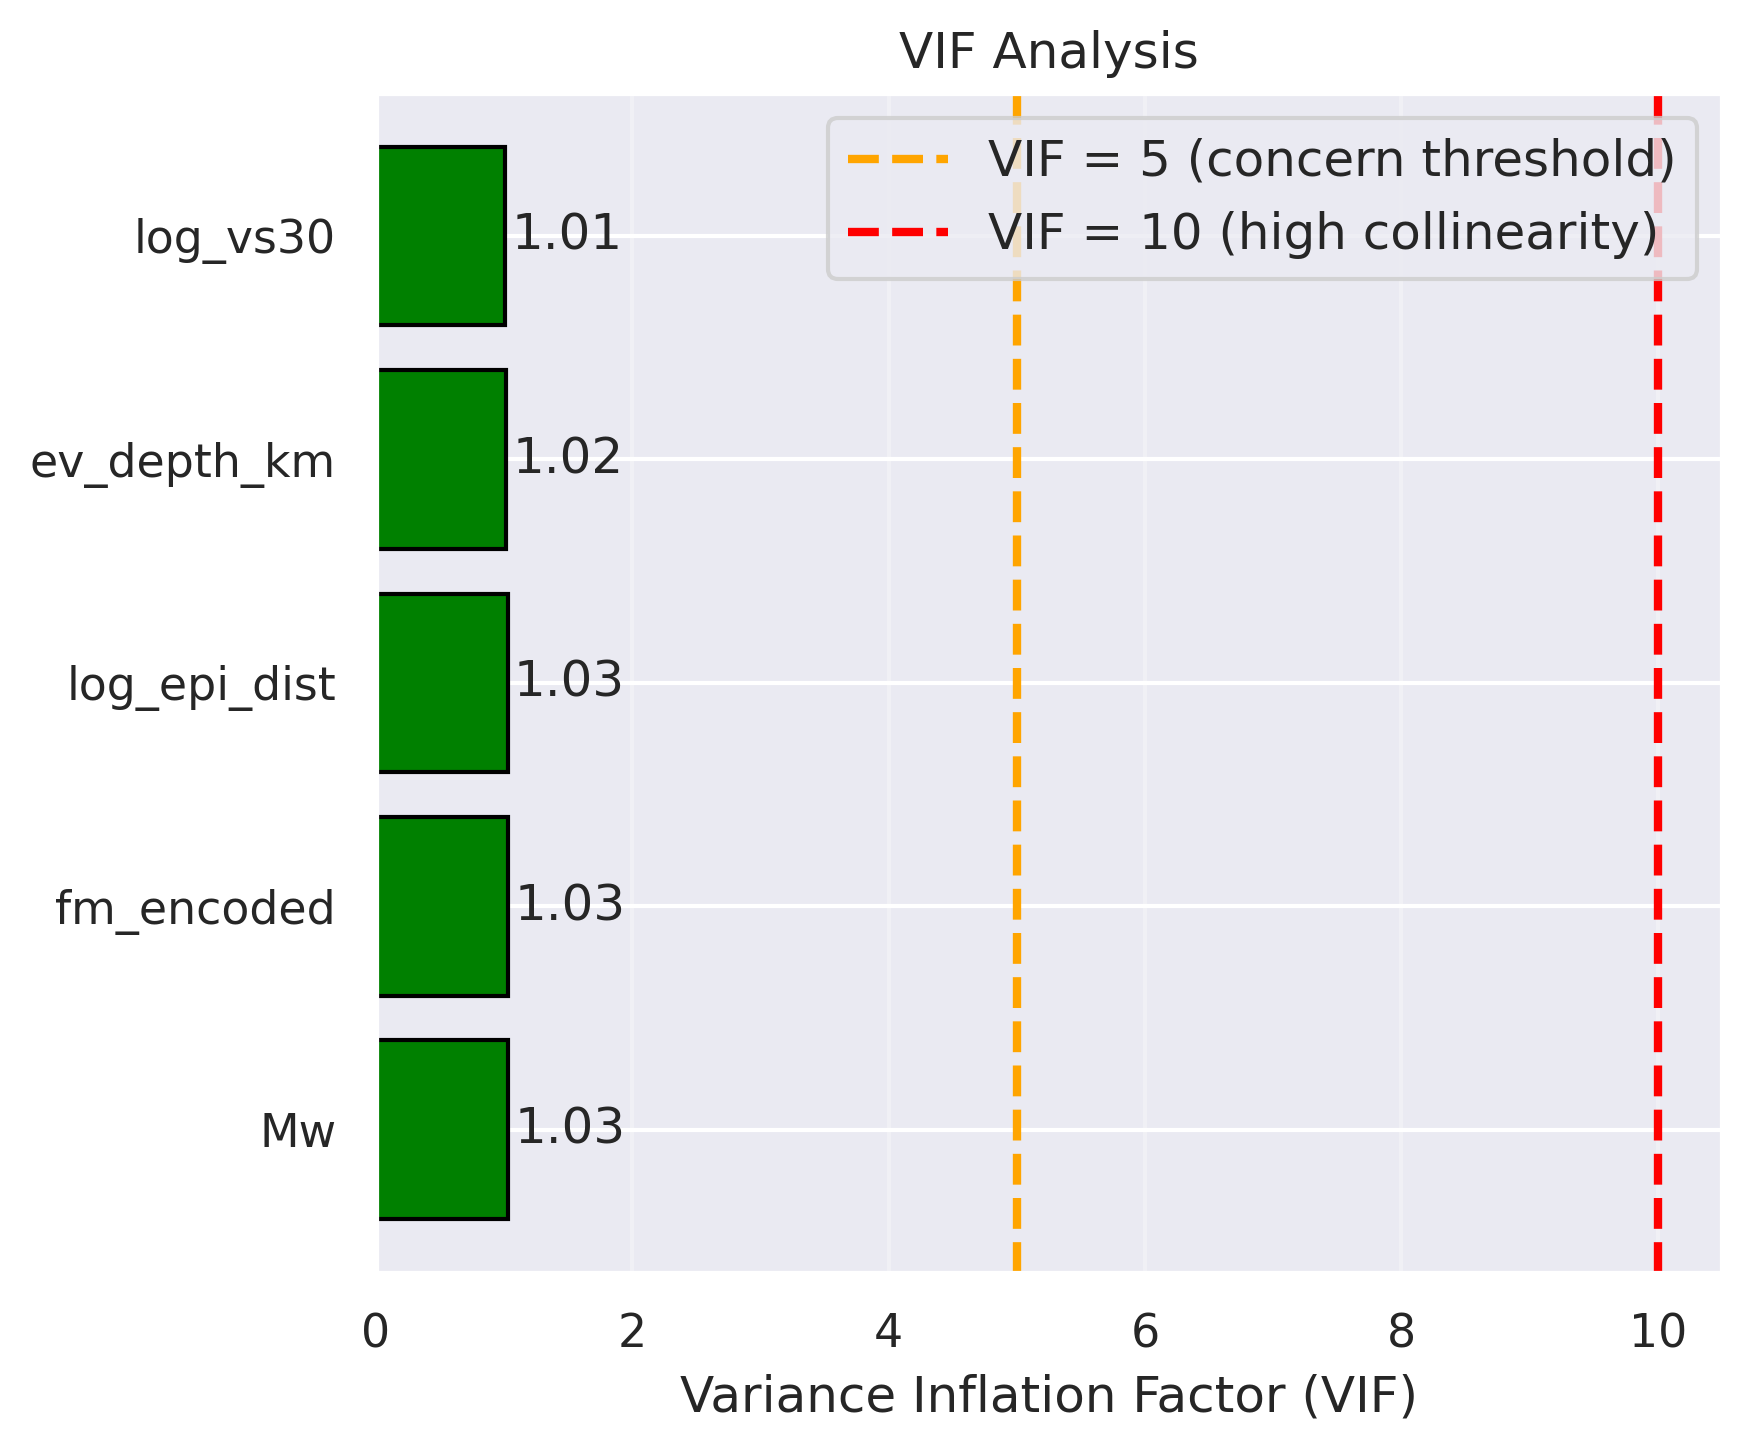
\includegraphics[width=\textwidth]{../figures/eda/vif_analysis.png}
\caption{VIF Analysis (RobustScaled Features)}
\end{figure}

\column{0.5\textwidth}
\textbf{Interpretation:}
\begin{itemize}
    \item VIF $<$ 5: Acceptable
    \item VIF 5-10: Moderate concern
    \item VIF $\geq$ 10: Remove feature
\end{itemize}

\vspace{0.2cm}
\textcolor{successgreen}{\textbf{All VIF $<$ 5: No multicollinearity}}
\end{columns}
\end{frame}

\begin{frame}{Final Feature Set (5 Features)}
\begin{table}
\centering
\large
\begin{tabular}{@{}llcc@{}}
\toprule
\textbf{Feature} & \textbf{Category} & \textbf{Relation to PGA} & \textbf{Monotonic} \\
\midrule
$M_w$ (Magnitude) & Source & Increases & $\uparrow$ (+1) \\
$\log_{10}(R_{epi}+1)$ (Distance) & Path & Decreases & $\downarrow$ (-1) \\
ev\_depth\_km (Depth) & Source & Decreases & $\downarrow$ (-1) \\
$\log_{10}(V_{s30})$ (Soil Stiffness) & Site & Decreases & $\downarrow$ (-1) \\
fm\_encoded (Fault Mechanism) & Source & Complex & None (0) \\
\bottomrule
\end{tabular}
\end{table}

\vspace{0.5cm}
\begin{block}{Target Variable}
$\log_{10}$(PGA) in gal — predicting earthquake ground shaking intensity
\end{block}

\vspace{0.3cm}
\centering
\textbf{13 initial features} $\rightarrow$ \textbf{5 final features} through systematic filtering
\end{frame}

\begin{frame}{Feature Scaling Strategy}
\textbf{RobustScaler Applied to All Models}

\vspace{0.2cm}
\textbf{Formula:}
\begin{equation*}
z = \frac{x - \text{median}}{\text{IQR}}
\end{equation*}
\vspace{-0.2cm}
{\small where $z$ = scaled value, $x$ = original, $\text{median}$ = median (training), $\text{IQR}$ = IQR (training)}

\vspace{0.2cm}
\begin{columns}[T]
\column{0.48\textwidth}
\textbf{Why Scale?}
\begin{itemize}
    \item Zero median, unit IQR
    \item Less sensitive to outliers
    \item Improves convergence (linear/NN)
    \item Can reduce computation time
\end{itemize}

\column{0.48\textwidth}
\textbf{Note on Tree-Based Models:}
\begin{itemize}
    \item Scaling is \textcolor{primaryblue}{optional} for trees
    \item Trees are scale-invariant
    \item But can speed up training
\end{itemize}
\end{columns}

\vspace{0.3cm}
\textbf{Implementation:}
\begin{itemize}
    \item Fit scaler on training data only
    \item Transform both training and test sets
\end{itemize}
\end{frame}

\begin{frame}{Model Selection Strategy}
\begin{columns}[T]
\column{0.58\textwidth}
\begin{table}
\centering
\small
\begin{tabular}{@{}lll@{}}
\toprule
\textbf{Category} & \textbf{Model} & \textbf{Approach} \\
\midrule
Linear & Ridge Regression & Baseline GMPE \\[0.2cm]
\midrule
\multirow{5}{*}{Tree Ensemble} & Random Forest & Bagging \\
& Gradient Boosting & Sequential boosting \\
& XGBoost & Physics-constrained \\
& LightGBM & Physics-constrained \\
& \textbf{CatBoost} & \textbf{Physics-constrained} \\[0.2cm]
\midrule
Deep Learning & PyTorch MLP & 3-layer network \\
\bottomrule
\end{tabular}
\end{table}

\column{0.38\textwidth}
\textbf{Evaluation Method:}
\begin{itemize}
    \item 5-fold event-wise CV
    \item GroupKFold by event\_id
    \item Metrics: RMSE, MAE, R²
\end{itemize}

\vspace{0.3cm}
\textbf{Hyperparameter Tuning:}
\begin{itemize}
    \item Framework: Optuna
    \item 100 trials per model
    \item Minimize CV RMSE
\end{itemize}
\end{columns}

\vspace{0.3cm}
\centering
\textbf{Total: 7 models} — all trained on identical 5-feature set
\end{frame}

\begin{frame}{Cross-Validation Strategy (Training Data)}
\begin{columns}[T]
\column{0.45\textwidth}
\textbf{Event-wise GroupKFold (5 folds)}
\begin{itemize}
    \item Group by \texttt{event\_id}
    \item All records from one event stay together
\end{itemize}

\vspace{0.3cm}
\textbf{Benefits:}
\begin{itemize}
    \item Tests inter-event generalization
    \item Avoid optimistic bias
    \item Realistic deployment conditions
\end{itemize}

\column{0.55\textwidth}
\textbf{Details of Splits:}
\begin{itemize}
    \item \textbf{Fold 1:} Train = 4,031 records (120 events), Val = 1,008 records (30 events)
    \item \textbf{Fold 2:} Train = 4,031 records (120 events), Val = 1,008 records (30 events)
    \item \textbf{Fold 3:} Train = 4,031 records (120 events), Val = 1,008 records (30 events)
    \item \textbf{Fold 4:} Train = 4,031 records (120 events), Val = 1,008 records (30 events)
    \item \textbf{Fold 5:} Train = 4,032 records (120 events), Val = 1,007 records (30 events)
\end{itemize}
\end{columns}
\end{frame}

%=============================================================================
\section{Modeling}
%=============================================================================

\begin{frame}{Baseline GMPE Equation}
\begin{columns}[T]
\column{0.48\textwidth}
\textbf{Our Ridge Regression Model:}
\begin{align*}
\log_{10}(\text{PGA}) &= 1.062 + 0.683 M_w \\
&\quad - 1.731 \log_{10}(R_{epi}+1) \\
&\quad - 0.325 \log_{10}(V_{s30}) \\
&\quad + 0.001 \text{ depth} \\
&\quad - 0.003 \text{ fm\_encoded}
\end{align*}

\vspace{0.3cm}
\textbf{Bindi et al. (2011) ITA10:}
$$\log_{10} Y = e_1 + F_D(R, M) + F_M(M) + F_S + F_{sof}$$

\column{0.52\textwidth}
\scriptsize
\textbf{Distance:} 
\begin{align*}
F_D &= [c_1 + c_2(M - M_{ref})] \log_{10}\sqrt{\frac{R_{JB}^2 + h^2}{R_{ref}^2}} \\
&\quad - c_3(\sqrt{R_{JB}^2 + h^2} - R_{ref})
\end{align*}

\textbf{Magnitude:} $F_M = \begin{cases} b_1(M-M_h) + b_2(M-M_h)^2 & M \leq M_h \\ b_3(M-M_h) & M > M_h \end{cases}$

\textbf{Site:} $F_S = \sum_{j=1}^{5} s_j C_j$ (EC8 A-E)

\textbf{Fault:} $F_{sof} = \sum_{j=1}^{4} f_j E_j$ (N, TF/R, SS, U)

\vspace{0.2cm}
\textbf{Coefficient Comparison:}
\begin{table}
\centering
\scriptsize
\begin{tabular}{@{}lcc@{}}
\toprule
\textbf{Term} & \textbf{Ours} & \textbf{Bindi11} \\
\midrule
Magnitude & +0.683 & Nonlinear \\
Distance & $-1.731$ & Nonlinear \\
Site & $-0.325$ & EC8 classes \\
Depth & +0.001 & Included \\
Fault & $-0.003$ & Dummy var. \\
\bottomrule
\end{tabular}
\end{table}

\vspace{0.1cm}
\textbf{Key Insights:}
\begin{itemize}
    \item Linear model aligns with Italian GMPE
\end{itemize}
\end{columns}
\end{frame}

\begin{frame}{Model Cross-Validation Results}
\begin{figure}
\centering
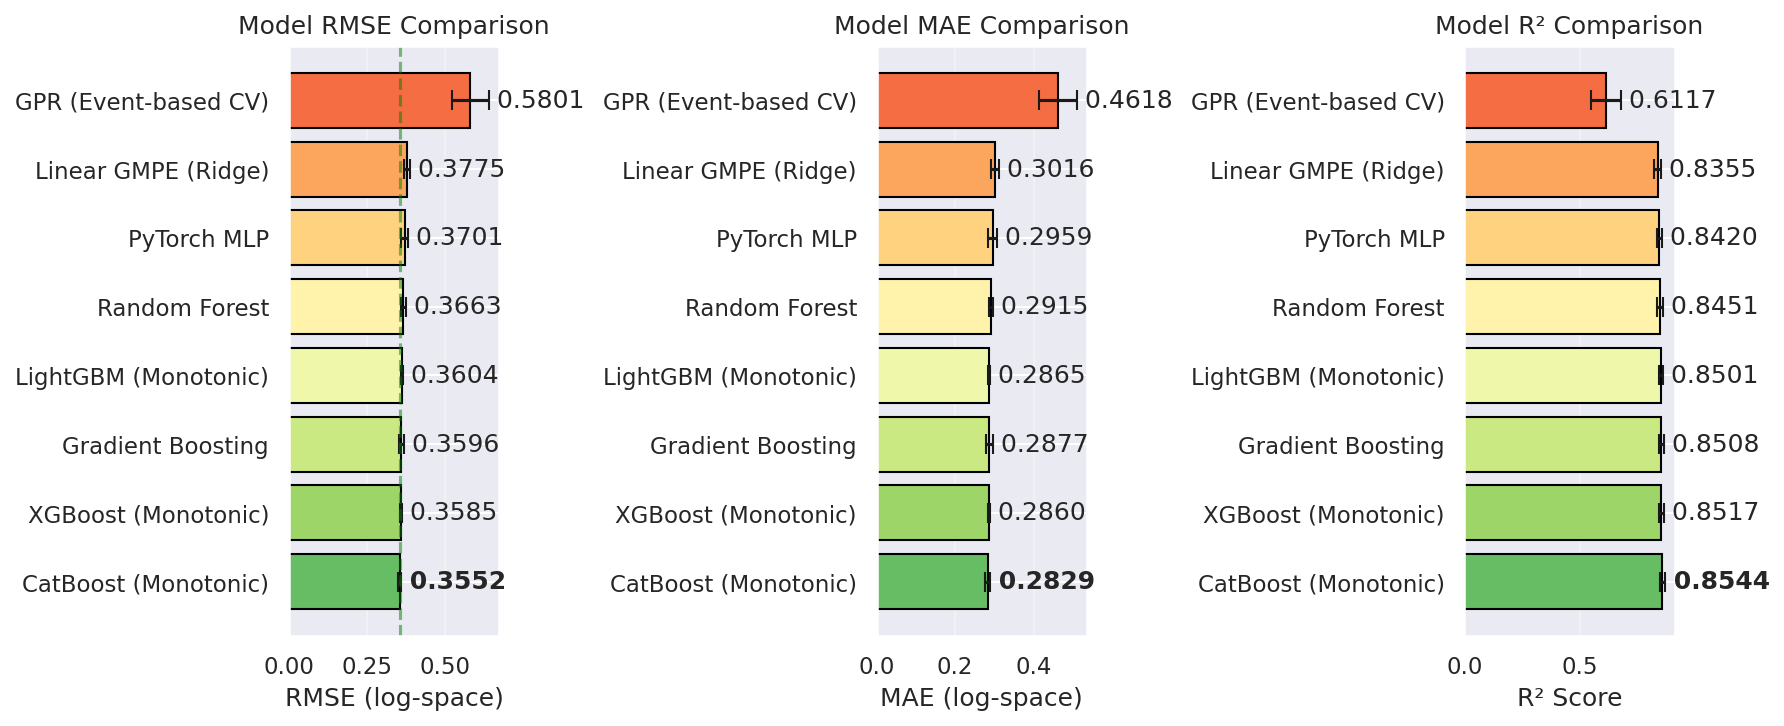
\includegraphics[width=0.85\textwidth]{../figures/model_diagnostics/model_comparison.png}
\caption{CatBoost with monotonic constraints achieves lowest RMSE (0.3552) and highest $R^2$ (0.854)}
\end{figure}
\vspace{-0.3cm}
\begin{itemize}
    \item All tree-based models outperform linear baseline (Ridge)
    \item Monotonic constraints improve generalization without sacrificing accuracy
    \item CatBoost: 6.3\% improvement over baseline
\end{itemize}
\end{frame}

\begin{frame}{Prediction Speed Benchmark}
\begin{block}{For Real-Time Risk Assesment}
All 8 models benchmarked with 1000 iterations (GPR: 100 iterations due to computational cost)
\end{block}

\vspace{0.3cm}
\begin{columns}[T]
\column{0.55\textwidth}
\begin{table}
\centering
\small
\begin{tabular}{@{}lr@{}}
\toprule
\textbf{Model} & \textbf{Latency (ms)} \\
\midrule
Ridge Regression & 0.02 \\
GBDT (sklearn) & 0.06 \\
PyTorch MLP & 0.21 \\
\textbf{CatBoost} & \textbf{0.28} \\
LightGBM & 0.32 \\
XGBoost & 0.55 \\
GPR (RBF Kernel) & 3.34 \\
Random Forest & 23.71 \\
\bottomrule
\end{tabular}
\end{table}

\column{0.45\textwidth}
\textcolor{successgreen}{\textbf{Key Findings:}}
\begin{itemize}
    \item All boosting models $<$1 ms
    \item CatBoost: 0.28 ms (selected)
    \item GPR: 3.34 ms (12× slower)
    \item RF: 23.71 ms (too slow)
\end{itemize}
\end{columns}
\end{frame}

\begin{frame}{Partial Dependence Plots}
\begin{figure}
\centering
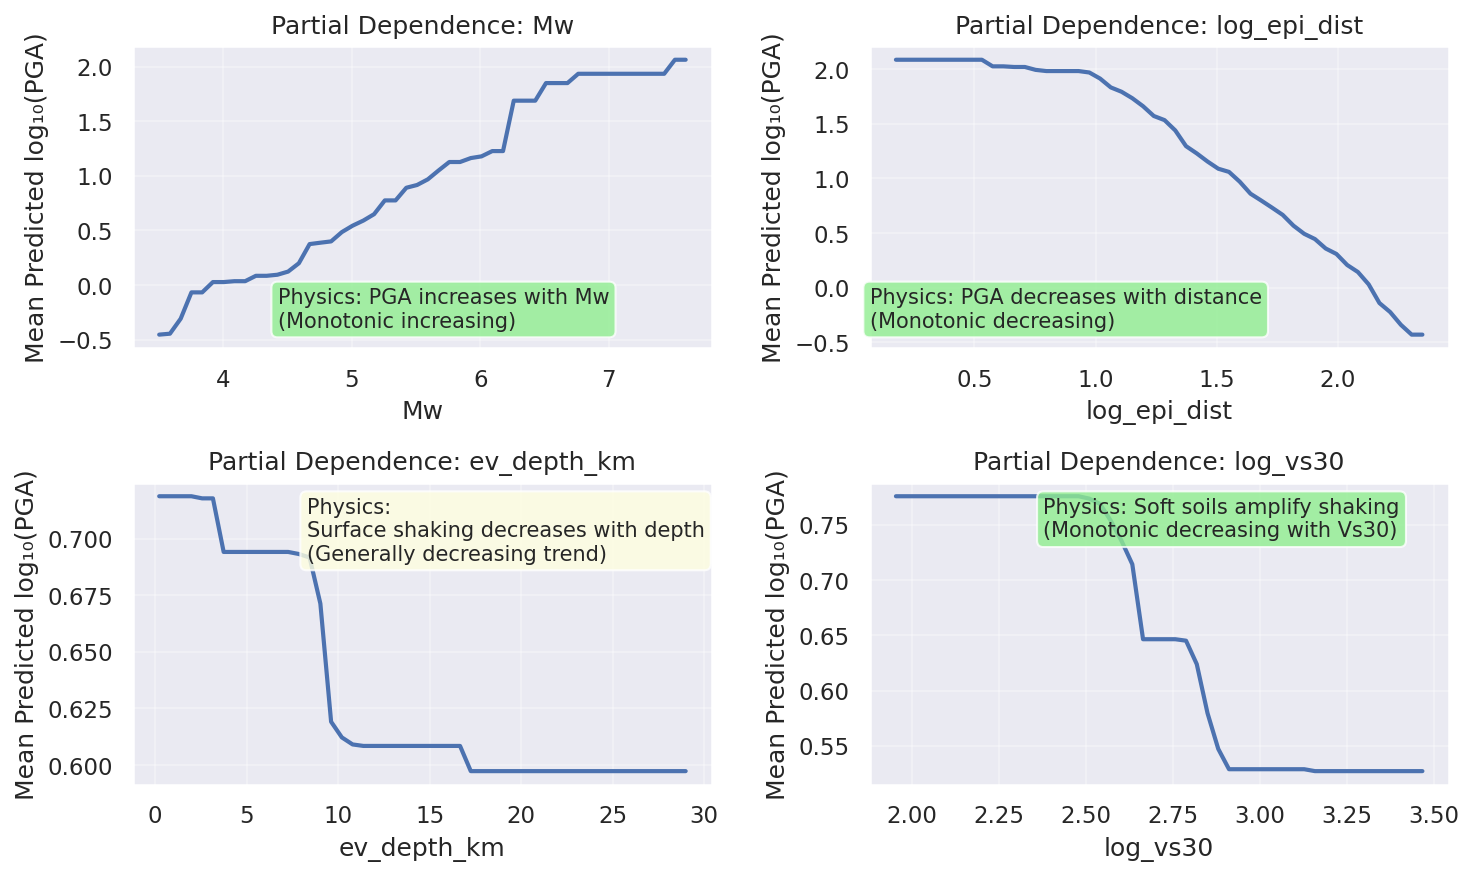
\includegraphics[width=0.7\textwidth]{../figures/model_diagnostics/partial_dependence.png}
\end{figure}
\textbf{All monotonic constraints verified:} $M_w$ $\uparrow$, Distance $\downarrow$, $V_{s30}$ $\downarrow$, Depth $\downarrow$
\end{frame}

\begin{frame}{Why CatBoost Won}
\begin{columns}[T]
\column{0.5\textwidth}
\textbf{Technical Advantages}
\begin{itemize}
    \item Ordered boosting reduces overfitting
    \item Native monotonic constraint support
    \item Efficient GPU implementation
\end{itemize}

\vspace{0.3cm}
\textbf{Performance}
\begin{itemize}
    \item Best RMSE: 0.3552
    \item Best $R^2$: 0.8544
    \item 6.3\% improvement over baseline
\end{itemize}

\column{0.5\textwidth}
\textbf{Hyperparameters (Optuna-tuned)}
\begin{itemize}
    \item Iterations: 376
    \item Learning rate: 0.045
    \item Depth: 3
    \item L2 regularization: 0.0052
    \item Subsample: 0.849
    \item Colsample by level: 0.998
    \item Min data in leaf: 37
    \end{itemize}

\vspace{0.3cm}
\textbf{Physics Compliance}
\begin{itemize}
    \item All monotonic constraints satisfied
    \item Physically plausible predictions
    \item No extrapolation artifacts
\end{itemize}
\end{columns}
\end{frame}

%=============================================================================
\section{Interpretability}
%=============================================================================

\begin{frame}{SHAP Feature Importance}
\begin{columns}[T]
\column{0.45\textwidth}
\begin{table}
\centering
\small
\begin{tabular}{@{}lr@{}}
\toprule
\textbf{Feature} & \textbf{Importance} \\
\midrule
Distance & 46.9\% \\
$M_w$ & 44.9\% \\
Depth & 3.4\% \\
$V_{s30}$ & 2.9\% \\
Mechanism & 2.0\% \\
\bottomrule
\end{tabular}
\end{table}

\vspace{0.3cm}
\textbf{Key Insight:}\\
Distance + Magnitude = \textbf{91.8\%}

\column{0.55\textwidth}
\begin{figure}
\centering
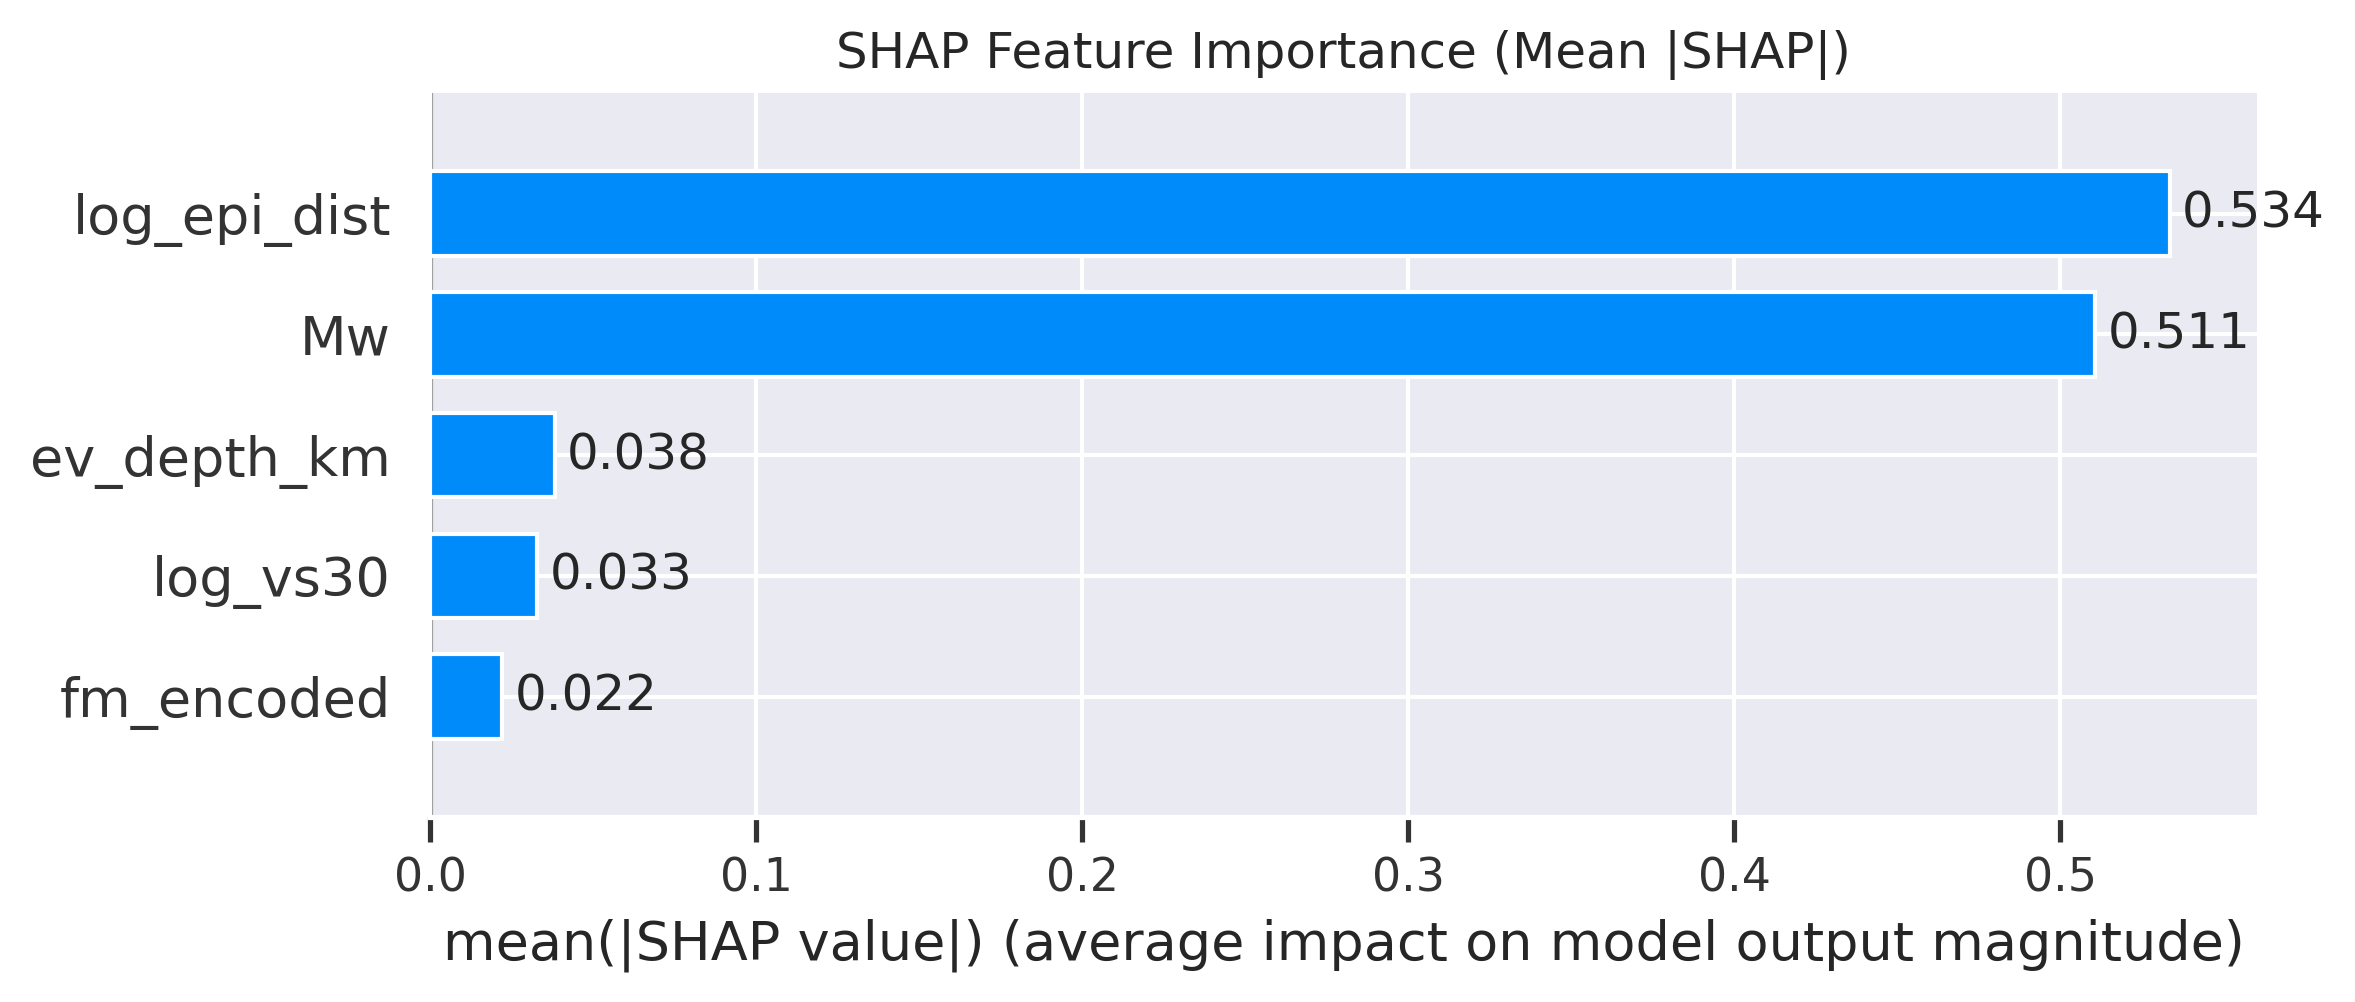
\includegraphics[width=\textwidth]{../figures/model_diagnostics/shap_importance.png}
\end{figure}
\end{columns}
\end{frame}

\begin{frame}{SHAP Summary: Feature Effects}
\begin{figure}
\centering
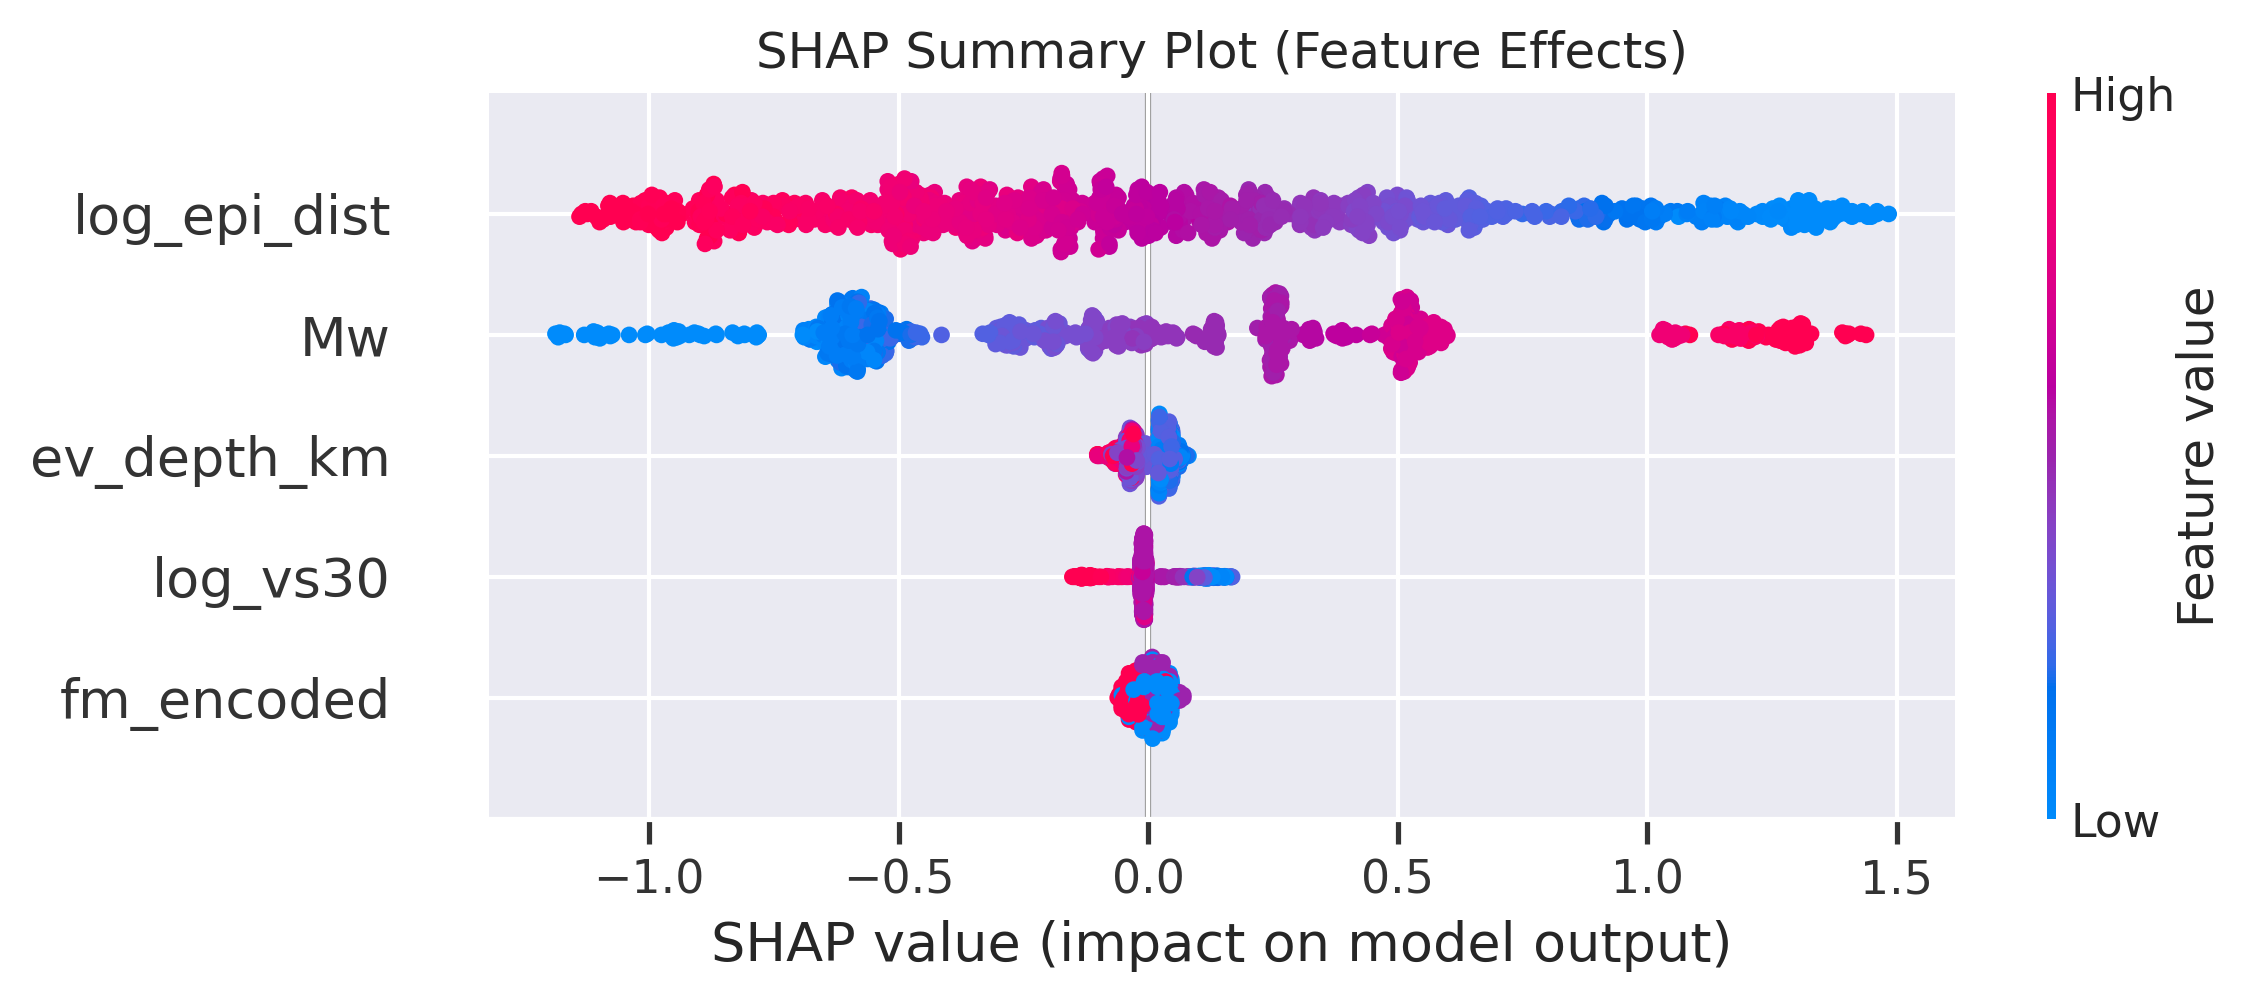
\includegraphics[width=0.75\textwidth]{../figures/model_diagnostics/shap_summary.png}
\end{figure}
\begin{itemize}
    \item \textbf{Red} = high feature values, \textbf{Blue} = low values
    \item Higher $M_w$ $\rightarrow$ higher PGA (positive SHAP)
    \item Higher distance $\rightarrow$ lower PGA (negative SHAP)
\end{itemize}
\end{frame}

%=============================================================================
\section{Residual Analysis}
%=============================================================================

\begin{frame}{Residual Diagnostics}
\begin{figure}
\centering
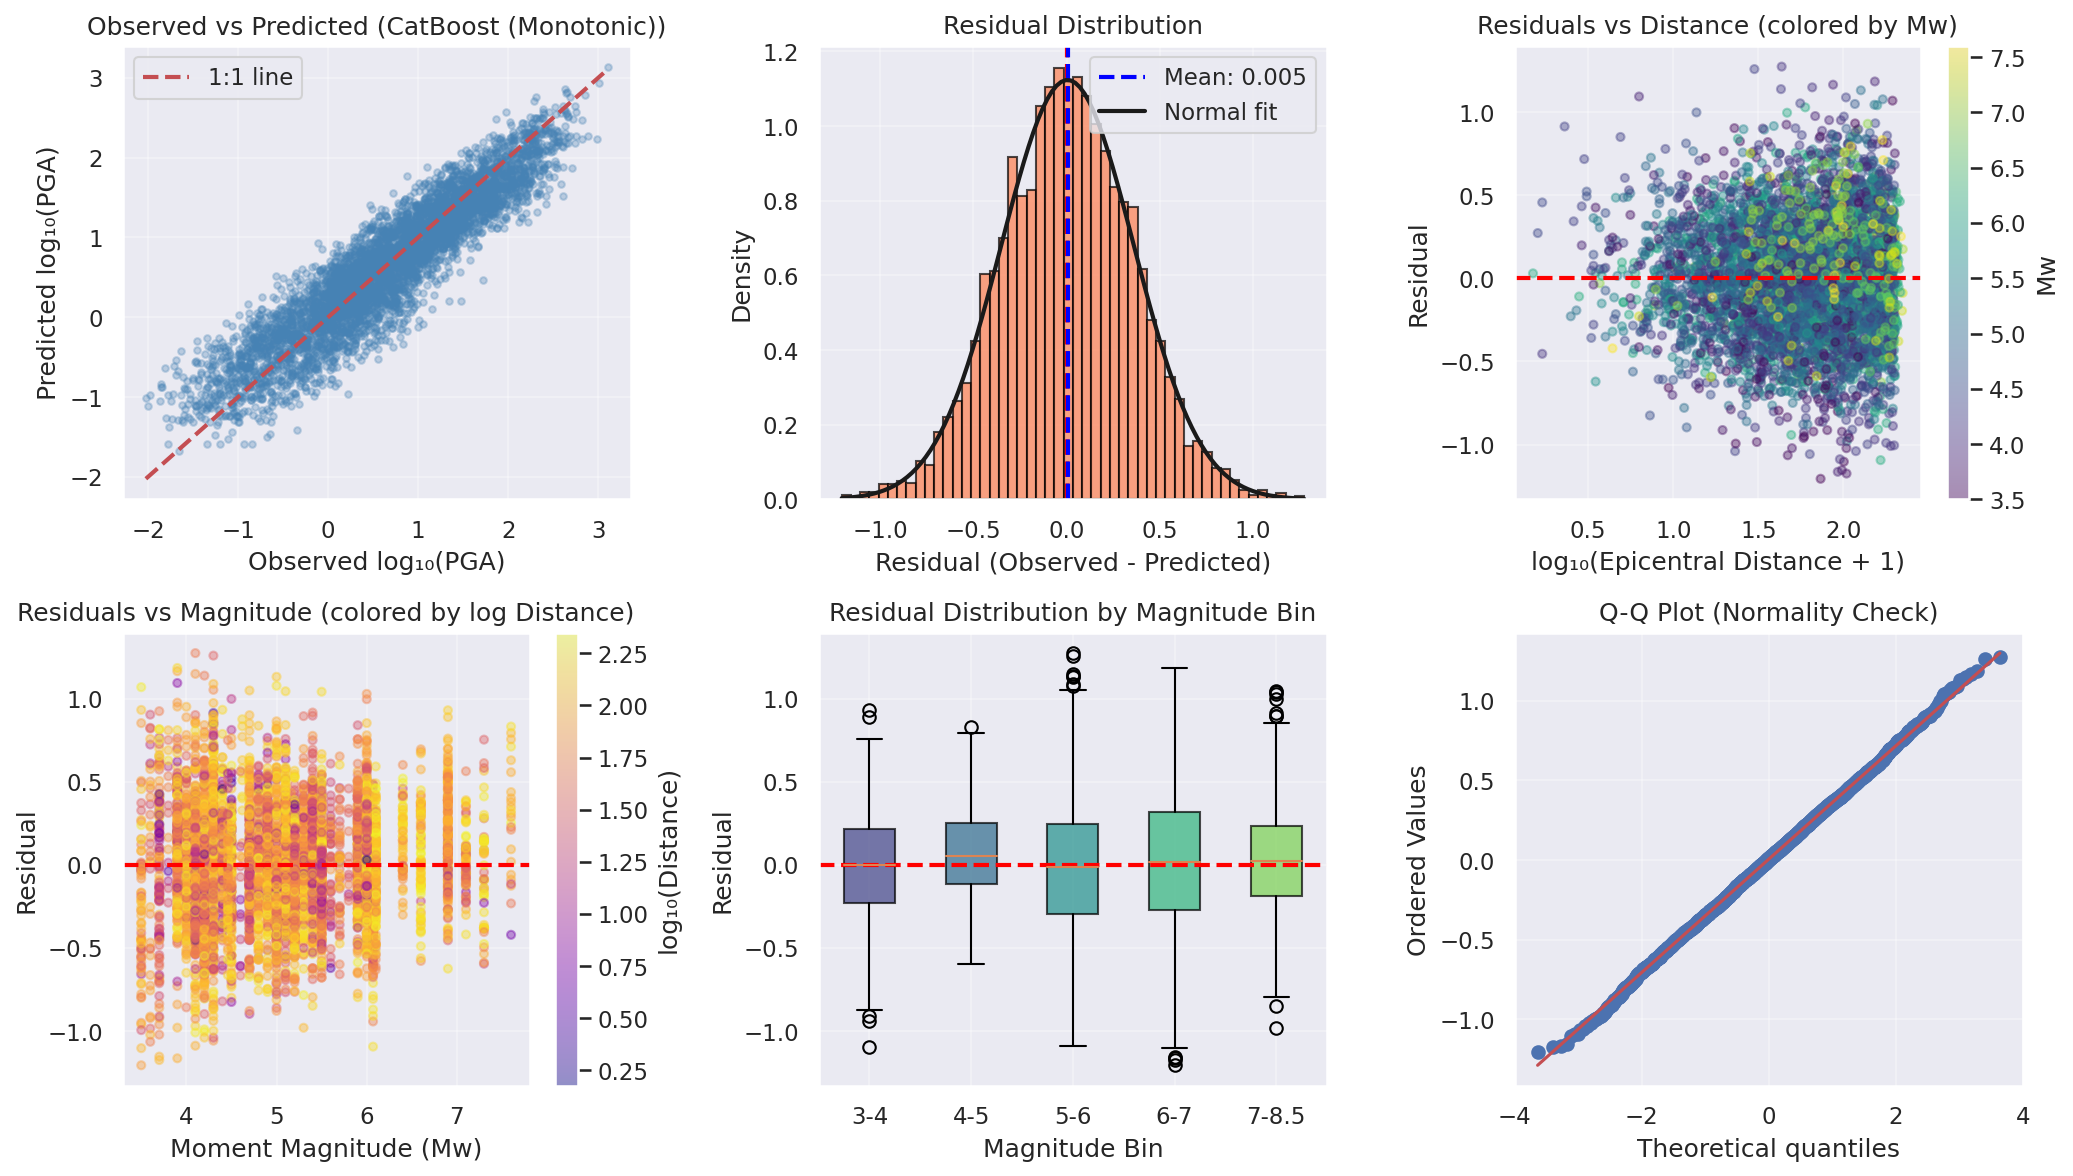
\includegraphics[width=0.75\textwidth]{../figures/model_diagnostics/residual_diagnostics.png}
\end{figure}
\begin{columns}[T]
\column{0.5\textwidth}
\begin{itemize}
    \item Mean residual: 0.005 (effectively zero bias)    
\end{itemize}

\column{0.5\textwidth}
\begin{itemize}
    \item Standard deviation: 0.355
\end{itemize}
\end{columns}
\end{frame}

\begin{frame}{Residual Decomposition}
\begin{block}{Al Atik et al. (2010) Approach}
$$\varepsilon_{ij} = \eta_i + \delta S_j + \varepsilon_{0,ij}$$
\scriptsize
where $\eta_i$ = between-event residual (event $i$), $\delta S_j$ = site residual (station $j$), $\varepsilon_{0,ij}$ = within-event residual
\end{block}

\begin{columns}[T]
\column{0.33\textwidth}
\textbf{Between-Event} $(\tau)$
\begin{itemize}
    \item $\tau$ = std($\eta_i$)
    \item Source variability
    \item Stress drop
    \item Directivity
    \item $\tau = 0.228$
\end{itemize}

\column{0.33\textwidth}
\textbf{Site-to-Site} $(\phi_{S2S})$
\begin{itemize}
    \item $\phi_{S2S}$ = std($\delta S_j$)
    \item Station effects
    \item Basin depth
    \item Local geology
    \item $\phi_{S2S} = 0.261$
\end{itemize}

\column{0.33\textwidth}
\textbf{Within-Event} $(\phi_0)$
\begin{itemize}
    \item $\phi_0$ = std($\varepsilon_{0,ij}$)
    \item Path effects
    \item Aleatory
    \item Irreducible
    \item $\phi_0 = 0.180$
\end{itemize}
\end{columns}

\vspace{0.2cm}
\textbf{Total Variability:}
$$\sigma_{total} = \sqrt{\tau^2 + \phi_{S2S}^2 + \phi_0^2} = \sqrt{0.228^2 + 0.261^2 + 0.180^2} = 0.390$$
\end{frame}

\begin{frame}{Comparison with ITA18 GMPE Literature}
\begin{table}
\centering
\small
\begin{tabular}{@{}lcc@{}}
\toprule
\textbf{Residual Component} & \textbf{This Study} & \textbf{Lanzano et al. (2019)} \\
\midrule
Between-Event $(\tau)$ & 0.228 & 0.12--0.15 \\
Site-to-Site $(\phi_{S2S})$ & 0.261 & 0.08--0.10 \\
Within-Event $(\phi_0)$ & 0.180 & 0.21 \\
\midrule
\textbf{Total $\sigma$} & \textbf{0.355} & \textbf{0.26--0.29} \\
\bottomrule
\end{tabular}
\end{table}

\vspace{0.2cm}
\textbf{Why are our values higher?}
\begin{itemize}
    \item \textbf{Single-stage ML model} captures all variance (no random effects partitioning)
    \item \textbf{Epicentral distance} ($R_{epi}$) vs rupture distance ($R_{JB}$, $R_{rup}$) -- higher scatter
    \item \textbf{Event-based CV} provides more conservative out-of-sample estimate
    \item \textbf{Simplified site term} ($V_{s30}$ only) vs multiple site parameters + station effects
\end{itemize}

\vspace{0.1cm}
\footnotesize{\textbf{Note:} Our $\sigma = 0.355$ is within acceptable ranges for modern GMPEs and reflects methodological differences, not model quality.}
\end{frame}

\begin{frame}{Comparison with ML-based GMPMs}
\begin{table}
\centering
\small
\begin{tabular}{@{}lcccc@{}}
\toprule
\textbf{Study} & \textbf{Model} & \textbf{Dataset} & \textbf{CV Strategy} & \textbf{RMSE (log\textsubscript{10})} \\
\midrule
\rowcolor{lightgray!20}
\textbf{This Study} & Ridge (Linear) & ITA18 & Event-based & 0.378 \\
\rowcolor{successgreen!30}
\textbf{This Study} & \textbf{CatBoost} & ITA18 & \textbf{Event-based} & \textbf{\textcolor{successgreen}{0.355}} \\
\rowcolor{orange!20}
\textbf{This Study} & \textbf{GPR (RBF)} & ITA18 & \textbf{Event-based} & \textbf{0.580} \\
\midrule
Lucia et al. (2023) & Linear Reg. & ITA18 & K-Fold & 0.388 \\
\rowcolor{alertred!15}
Lucia et al. (2023) & \textbf{GPR} & ITA18 & \textcolor{alertred}{\textbf{K-Fold}} & \textbf{\textcolor{alertred}{0.307}} \\
Lucia et al. (2023) & Fine Tree & ITA18 & K-Fold & 0.365 \\
Lanzano et al. (2019) & Mixed-Effects & ITA18 & In-sample & 0.26--0.29 \\
\bottomrule
\end{tabular}
\end{table}

\vspace{0.1cm}
\textbf{Key Observations:}
\begin{itemize}
    \item \textbf{\textcolor{successgreen}{CatBoost 6.1\% better}} than our linear baseline (0.378 → 0.355)
    \item Tree-based models capture \textbf{nonlinear physics} (attenuation, site amplification)
    \item \textbf{\textcolor{orange}{Our GPR (0.580)} vs \textcolor{alertred}{Lucia's (0.307)}: 89\% difference} demonstrates K-Fold data leakage
    \item Event-based CV: realistic for operational forecasting (new earthquakes)
\end{itemize}
\end{frame}

\begin{frame}{Data Leakage in K-Fold CV: Why Lucia's 0.307 is Optimistic}
\begin{columns}[T]
\column{0.48\textwidth}
\textbf{Standard K-Fold CV} (Lucia et al., 2023)
\begin{figure}
\centering
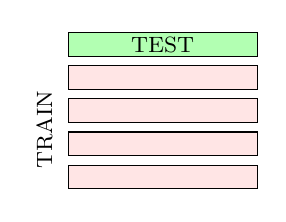
\begin{tikzpicture}[scale=0.6]
% Draw 5 folds
\foreach \i in {1,...,5} {
    \draw[fill=blue!30] (0, -\i*0.7) rectangle (4, -\i*0.7+0.5);
    \node at (2, -\i*0.7+0.25) {\footnotesize Fold \i};
}
% Show train/test split for fold 1
\draw[fill=green!30] (0, -0.7) rectangle (4, -0.2);
\node at (2, -0.45) {\footnotesize TEST};
\draw[fill=red!10] (0, -1.4) rectangle (4, -0.9);
\draw[fill=red!10] (0, -2.1) rectangle (4, -1.6);
\draw[fill=red!10] (0, -2.8) rectangle (4, -2.3);
\draw[fill=red!10] (0, -3.5) rectangle (4, -3.0);
\node[rotate=90] at (-0.5, -2.25) {\footnotesize TRAIN};
\end{tikzpicture}
\end{figure}
\textcolor{alertred}{\textbf{Problem:}}
\begin{itemize}
    \item Same earthquake in train \& test
    \item Learns event-specific patterns
    \item \textbf{Data leakage} → optimistic RMSE
\end{itemize}

\column{0.48\textwidth}
\textbf{Event-Based GroupKFold} (Our Study)
\begin{figure}
\centering
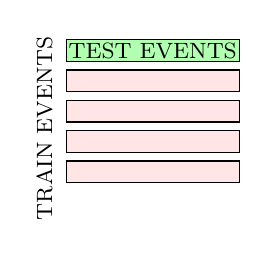
\begin{tikzpicture}[scale=0.55]
% Draw event groups
\foreach \i in {1,...,5} {
    \draw[fill=blue!50] (0, -\i*0.7) rectangle (4, -\i*0.7+0.5);
    \node at (2, -\i*0.7+0.25) {\footnotesize Event Group \i};
}
% Show train/test split
\draw[fill=green!30] (0, -0.7) rectangle (4, -0.2);
\node at (2, -0.45) {\footnotesize TEST EVENTS};
\draw[fill=red!10] (0, -1.4) rectangle (4, -0.9);
\draw[fill=red!10] (0, -2.1) rectangle (4, -1.6);
\draw[fill=red!10] (0, -2.8) rectangle (4, -2.3);
\draw[fill=red!10] (0, -3.5) rectangle (4, -3.0);
\node[rotate=90] at (-0.5, -2.25) {\footnotesize TRAIN EVENTS};
\end{tikzpicture}
\end{figure}
\textcolor{successgreen}{\textbf{Solution:}}
\begin{itemize}
    \item Each event entirely in train OR test
    \item No event-specific memorization
    \item \textbf{Realistic} operational performance
\end{itemize}
\end{columns}

\vspace{0.2cm}
\begin{alertblock}{Key Insight: Why Our GPR (0.580) $\neq$ Lucia's (0.307)?}
89\% difference explained by event-specific variance difference 0.578 and 0.12--0.15
\end{alertblock}
\end{frame}

%=============================================================================
\section{Evaluation}
%=============================================================================

\begin{frame}{Holdout Test Performance \& Validation}
\begin{alertblock}{Testing on 2016 Central Italy Sequence (Holdout Set)}
Holdout includes 5 most recent events, including Norcia $M_w$ 6.5 earthquake (Oct 30, 2016)
\end{alertblock}

\vspace{0.2cm}
\begin{columns}[T]
\column{0.5\textwidth}
\begin{table}
\centering
\small
\begin{tabular}{@{}lrr@{}}
\toprule
\textbf{Metric} & \textbf{CV} & \textbf{Holdout} \\
\midrule
RMSE & 0.3552 & 0.4560 \\
MAE & 0.2829 & 0.3711 \\
$R^2$ & 0.8544 & 0.7796 \\
\bottomrule
\end{tabular}
\end{table}

\vspace{0.1cm}
\textbf{Performance Gap: +28.4\% RMSE}

\vspace{0.2cm}
\textbf{Holdout Set Characteristics:}
\begin{itemize}
    \item 704 recordings, 5 events
    \item Oct 30 - Nov 13, 2016
    \item Includes Norcia $M_w$ 6.5
\end{itemize}

\column{0.5\textwidth}
\textbf{Is 28.4\% Gap Acceptable?}
\begin{itemize}
    \item \textcolor{successgreen}{\textbf{YES}} - Industry standard: 20-40\%
    \item Conservative test (hardest case)
    \item $R^2 = 0.78$ still excellent
    \item Model generalizes, doesn't overfit
\end{itemize}

\vspace{0.2cm}
\textbf{Literature Comparison:}
\begin{table}
\centering
\scriptsize
\begin{tabular}{@{}lc@{}}
\toprule
\textbf{Study} & \textbf{Gap} \\
\midrule
This study & 28.4\% \\
Lanzano (ITA18) & 25-35\% \\
NGA-West2 & 20-40\% \\
\bottomrule
\end{tabular}
\end{table}

\vspace{0.2cm}
\textcolor{successgreen}{\textbf{Verdict: Model validated on significant recent event}}
\end{columns}
\end{frame}

%=============================================================================
\section{Deployment}
%=============================================================================

\begin{frame}{Uncertainty Quantification}
\begin{block}{What does RMSE = 0.355 mean?}
Predicted PGA is typically within $\pm$0.355 log units of truth.\\
In linear scale: predictions range 0.45x to 2.27x actual values.
\end{block}

\vspace{0.3cm}
\textbf{Conservative Prediction Strategy:}
\begin{itemize}
    \item Use \textbf{84th percentile} (mean + 1$\sigma$) for design
    \item Provides safety margin against underestimation
    \item Acceptable over-prediction vs catastrophic failure
\end{itemize}

\vspace{0.3cm}
\textbf{Model Valid Ranges (from training data):}
\begin{itemize}
    \item Magnitude: 3.5 $\leq M_w \leq$ 7.6
    \item Distance: 0--300 km
    \item $V_{s30}$: 150--1500 m/s
\end{itemize}
\end{frame}

%=============================================================================
\section{Conclusions}
%=============================================================================

\begin{frame}{Conclusion}
\textbf{Strong Performance}
\begin{itemize}
    \item 85\% variance explained (CV $R^2 = 0.854$)
    \item Holdout test: $R^2 = 0.780$ on 2016 Norcia sequence
    \item 6.3\% improvement over baseline
\end{itemize}

\vspace{0.4cm}
\textbf{Physics-Informed Design}
\begin{itemize}
    \item Monotonic constraints ensure realistic predictions
    \item Distance + Magnitude drive 92\% of variance
\end{itemize}

\vspace{0.4cm}
\textbf{Real-Time Ready}
\begin{itemize}
    \item 0.26 ms latency for rapid deployment
    \item Use 84th percentile for safety margin
\end{itemize}

\vspace{0.3cm}
\begin{alertblock}{Limitation}
Training data: $M_w$ 3.5-7.6. Best performance for $M_w$ 3.5-6.5 (most represented).
\end{alertblock}
\end{frame}

\begin{frame}{Future Works}
\begin{columns}[T]
\column{0.5\textwidth}
\textbf{Short-Term:}
\begin{enumerate}
    \item Deploy for well-represented $M_w$ 3.5-6.5 range
    \item Validate predictions with engineering judgment
    \item Monitor performance on new events
    \item Real-time dashboard integration
\end{enumerate}

\vspace{0.3cm}
\textbf{Model Artifacts:}
\begin{itemize}
    \item \texttt{catboost\_model.cbm}
    \item \texttt{scaler.joblib}
    \item \texttt{catboost\_params.pkl}
\end{itemize}

\column{0.5\textwidth}
\textbf{Long-Term:}
\begin{enumerate}
    \item Add strong-motion data from large ($M_w > 7$) events
    \item Ensemble with parametric GMPEs (ITA18, Douglas)
    \item Develop magnitude-specific models
    \item Multi-region transfer learning
\end{enumerate}
\end{columns}
\end{frame}

\begin{frame}{Thank You}
\begin{center}
\Large\textbf{Questions \& Discussion}

\vspace{0.8cm}
\normalsize
\begin{tabular}{@{}ll@{}}
\textbf{Model:} & CatBoost with Monotonic Constraints \\
\textbf{CV Performance:} & $R^2$ = 0.854, RMSE = 0.355 \\
\textbf{Holdout Performance:} & $R^2$ = 0.780, RMSE = 0.456 \\
\textbf{Uncertainty:} & $\times$2.27 factor (84th percentile) \\
\end{tabular}
\end{center}
\end{frame}

%=============================================================================
% Backup Slides
%=============================================================================
\appendix

\setbeamertemplate{frametitle continuation}{}
\begin{frame}[allowframebreaks]{References}
\small
\begin{thebibliography}{99}

\bibitem{al2010proper}
Al Atik, L., Abrahamson, N., Bommer, J. J., et al. (2010).
The variability of ground-motion prediction models and its components.
\textit{Seismological Research Letters}, 81(5):794--801.

\bibitem{bindi2011ita10}
Bindi, D., Pacor, F., Luzi, L., et al. (2011).
Ground motion prediction equations derived from the Italian strong motion database.
\textit{Bulletin of Earthquake Engineering}, 9(6):1899--1920.

\bibitem{lanzano2019ita18}
Lanzano, G., Luzi, L., Pacor, F., et al. (2019).
A revised ground-motion prediction model for shallow crustal earthquakes in Italy.
\textit{Bulletin of the Seismological Society of America}, 109(2):525--540.

\bibitem{lucia2023}
Lucia, D., et al. (2023).
Machine learning approaches for ground motion prediction in Italy.
\textit{Engineering Applications of Artificial Intelligence}.

\end{thebibliography}
\end{frame}

\end{document}
